\documentclass{article}

% NeurIPS 2026 style. Default (no options) = main-track, double-blind, anonymous submission.
% For camera-ready, switch to: \usepackage[main, final]{neurips_2026}
% For arXiv preprint,         switch to: \usepackage[preprint]{neurips_2026}
\usepackage{neurips_2026}
\usepackage[utf8]{inputenc}
\usepackage[T1]{fontenc}
\usepackage{hyperref}
\usepackage{url}
\usepackage{booktabs}
\usepackage{amsfonts}
\usepackage{nicefrac}
\usepackage{microtype}
\usepackage[table]{xcolor}
\usepackage{graphicx}
\usepackage{overpic}
\usepackage{multirow}
\usepackage{amsmath}
\usepackage{amssymb}
\usepackage{mathtools}
\usepackage{amsthm}
\usepackage{algorithm}
\usepackage{algpseudocode}
\newcommand{\theHalgorithm}{\arabic{algorithm}}
\usepackage[capitalize,noabbrev]{cleveref}
\usepackage{colortbl}
\theoremstyle{plain}
\newtheorem{theorem}{Theorem}[section]
\newtheorem{proposition}[theorem]{Proposition}
\newtheorem{lemma}[theorem]{Lemma}
\newtheorem{corollary}[theorem]{Corollary}
\theoremstyle{definition}
\newtheorem{definition}[theorem]{Definition}
\newtheorem{assumption}[theorem]{Assumption}
\theoremstyle{remark}
\newtheorem{remark}[theorem]{Remark}
\usepackage[textsize=tiny]{todonotes}
\usepackage{wrapfig}
\usepackage{subcaption}

% Shortcuts
\newcommand{\tsimg}{\texttt{ts\_to\_img}}
\newcommand{\imgts}{\texttt{img\_to\_ts}}
\newcommand{\Nts}{N_{\mathrm{ts}}}
\newcommand{\Nimg}{N_{\mathrm{img}}}
\newcommand{\Nobs}{N_{\mathrm{obs}}}
\newcommand{\Ats}{A_{\mathrm{ts}}}
\newcommand{\Aimg}{A_{\mathrm{img}}}
\newcommand{\yts}{y_{\mathrm{ts}}}
\newcommand{\xts}{x_{\mathrm{ts}}}
\newcommand{\ximg}{x_{\mathrm{img}}}

\title{Posterior Sampling in Lifted Representations for \\ Corrupted Time Series Generation}

\author{%
  Anonymous Authors \\
  Anonymous Affiliation \\
  \texttt{anonymous@email.edu} \\
}

\begin{document}

\maketitle

\begin{abstract}
State-of-the-art time series generation operates in a \emph{lifted representation}: delay embedding maps time series to images, and standard image diffusion is applied in image space. When training data is corrupted by missing values, this creates a \emph{dual-space} system where observations live in time-series space while the generative model operates in image space. A natural framework for this regime is Expectation-Maximization: alternate between imputing missing data using the model's prior (E-step) and training on those imputations (M-step). However, the natural combination of DiEM's EM loop with ImagenTime's delay embedding fails out of the box, because the Moment-Matching Posterior Sampling (MMPS) derivation assumes an observation operator that acts in the model's native space. We identify \emph{posterior misspecification in lifted representations} as a general problem class and prove a convergence theorem showing that operator mismatch in the E-step determines whether MCEM converges, diverges, or stagnates. Guided by the theorem, we introduce four principled E-step corrections---observation-space conjugate gradient ($\sim 28\times$ dimensionality reduction), adaptive $\sigma_y$, manifold projection, and domain-aware initialization---which together add exactly one tuned hyperparameter to vanilla EM. On Energy 50\% missing, our method achieves discriminative score $0.045$---within $1.3\%$ of the clean-data oracle ($0.044$)---converging in $3$ EM iterations. Alternative E-steps collapse catastrophically (DPS: $0.500$; PiGDM: $0.462$), and the strongest frozen stochastic imputer (CSDI-impute $+$ EDM: $0.105$) is beaten even by vanilla EM with the \emph{wrong} operator ($0.092$), showing that iteration, not imputer sophistication, is the binding constraint. The three predicted convergence regimes are validated on two structurally different linear lifts (delay embedding and STFT), confirming that the operator-mismatch principle is lift-agnostic.
\end{abstract}

\vspace{-3mm}
\section{Introduction}
\label{sec:intro}
\vspace{-1mm}

State-of-the-art time series generation operates in a \emph{lifted representation}: delay embedding maps time series to images, and standard image diffusion \citep{karras2022edm} is applied in image space~\citep{naiman2024imagentime}. When the training data is corrupted---sensors fail, measurements are intermittent, records have gaps---this creates a \emph{dual-space} system: observations live in time-series space while the generative model operates in image space.

Learning from corrupted data naturally calls for Expectation-Maximization \citep{dempster1977em}: alternate between completing missing data using the model's learned prior (E-step) and training on those completions (M-step). DiEM \citep{rozet2024diem} demonstrated this framework for image reconstruction with MMPS posterior sampling. The combination---DiEM's EM loop applied to ImagenTime's delay-embedding pipeline---is the natural starting point.

\paragraph{The problem we solve.}
This combination fails out of the box. The E-step requires posterior sampling conditioned on \emph{time-series-space} observations, but MMPS was derived for single-space settings where the observation operator acts in the model's native space. In the dual-space setting, MMPS is structurally misspecified: it uses the wrong observation operator, suffers unbounded CG conditioning, and produces off-manifold outputs. Vanilla EM with standard MMPS achieves discriminative score $0.092$ on Energy $50\%$---far from the $0.05$ SOTA target.

We identify \emph{posterior misspecification in lifted representations} as a general problem class arising whenever EM operates in a representation different from the observation space, and provide four principled corrections that reduce the discriminative score to $0.045$---a $51\%$ improvement over vanilla EM. Alternative E-step methods fail dramatically: DPS (point estimate) achieves $0.500$ (random chance) and PiGDM (diagonal covariance) achieves $0.462$---confirming that full Jacobian covariance with the \emph{correct} operator is essential. Our result is within $1.3\%$ of the \emph{clean-data oracle} ($0.044$, trained on fully observed data), meaning EM with the corrected E-step recovers nearly all information lost to $50\%$ corruption. The method achieves state-of-the-art across datasets, missing rates, and missingness patterns, converging in $3$ EM iterations.

\paragraph{Why EM over commit-and-forget?}
All existing methods for corrupted time series generation---GT-GAN \citep{jeon2022gtgan}, KoVAE \citep{naiman2024kovae}, ImagenI2R \citep{fadlon2025imageni2r}---follow a \emph{commit-and-forget} pattern: one-shot imputation, then frozen training. The imputer never receives feedback from the generator. We show (\cref{sec:why-close}) that this introduces systematic variance collapse---a well-known phenomenon in multiple imputation \citep{rubin1987multiple}---and a masking--data trade-off at high missing rates. Strikingly, even stochastic commit-and-forget with a strong dedicated imputer fails to match iterative EM: CSDI-impute $+$ EDM \citep{tashiro2021csdi} achieves $0.105$, \emph{worse} than vanilla EM with the wrong observation operator ($0.092$), and $2.3\times$ worse than our full method ($0.045$). Iteration---not imputer sophistication---is the binding constraint.

\begin{table}[t]
\centering
\caption{Existing paradigms for corrupted time-series generation. All follow commit-and-forget.}
\label{tab:intro-taxonomy}
\resizebox{0.95\textwidth}{!}{
\begin{tabular}{l l l l l}
\toprule
\textbf{Family} & \textbf{Representative} & \textbf{Imputer} & \textbf{Generator} & \textbf{Limitation} \\
\midrule
GAN-based & GT-GAN \citep{jeon2022gtgan} & Neural CDE (one-shot) & GAN & Unstable, mode collapse \\
VAE-based & KoVAE \citep{naiman2024kovae} & Neural CDE (one-shot) & Koopman VAE & $\sim 6.5\times$ slower, limited expressiveness \\
Diffusion-based & ImagenI2R \citep{fadlon2025imageni2r} & TST (one-shot, det.) & Masked diffusion & Masking--data trade-off \\
Diffusion-based & CSDI-impute $+$ EDM & CSDI (one-shot, stoch.) & Standard diffusion & Frozen imputer, no generator feedback \\
\bottomrule
\end{tabular}
}
\vspace{-3mm}
\end{table}

\paragraph{Contributions.}
\begin{enumerate}
\setlength{\itemsep}{0pt}
\item \textbf{Problem identification.} We identify \emph{posterior misspecification} as the core obstacle to EM in lifted representations: three structural misspecifications of MMPS in the dual-space setting (wrong operator, unbounded conditioning, off-manifold drift), each arising because MMPS assumes a single-space observation model. This problem class applies beyond delay embedding to any representation-based EM (latent diffusion, spectral lifts).
\item \textbf{Convergence theory (Theorem~\ref{thm:operator-mismatch}).} We prove that the choice of observation operator in the E-step determines whether MCEM converges, diverges, or stagnates. For linear-Gaussian MCEM with operator mismatch $\Delta$: (a) $\Delta = 0$ guarantees contraction to the ML estimate; (b) small $\|\Delta\|$ causes initial convergence followed by divergence at a predictable iteration $k^\star$; (c) large $\|\Delta\|$ traps iterates at a biased fixed point. The four E-step corrections are the necessary steps to achieve $\Delta = 0$; the theorem explains \emph{why} each is needed, not just \emph{that} it helps.
\item \textbf{E-step corrections.} Four principled adaptations of MMPS for dual-space EM---observation-space CG with $\sim 28\times$ dimensionality reduction, adaptive $\sigma_y$ for bounded CG conditioning, manifold projection, and domain-aware initialization---yielding a method with exactly one \emph{tuned} hyperparameter beyond vanilla EM ($c$ in $\sigma_y = c\,\sigma_t$), all other knobs fixed at defaults and audited in Algorithms~\ref{alg:estep}--\ref{alg:em} (App.~\ref{app:algorithms}), and standard score matching in the M-step.
\item \textbf{EM framework for corrupted time series.} The first application of EM to corrupted time series generation. We provide a formal analysis of why stochastic co-evolution outperforms commit-and-forget (variance collapse, masking trade-off), confirmed by a controlled $2$D experiment that separates the benefit of stochastic sampling from the benefit of iterative refinement.
\item \textbf{SOTA results.} State-of-the-art generation quality across five datasets, three missing rates, extended sequence lengths, structured missingness patterns, and a $50\times$-wide robust band for the one tuned hyperparameter. On Energy $50\%$, our corrected EM achieves $0.045$---within $1.3\%$ of the clean-data oracle ($0.044$), converging in $3$ EM iterations. On Weather $70\%$, $0.038$; under block missing at $50\%$, $0.069$.
\item \textbf{Generality across lifts.} We validate the theorem's predictions on two structurally different linear lifts---delay embedding (spatial redundancy) and STFT (frequency-domain redundancy)---confirming that the three convergence regimes are lift-agnostic (App.~\ref{app:stft}).
\end{enumerate}

\vspace{-2mm}
\section{Related Work}
\label{sec:related}
\vspace{-1mm}

\paragraph{Corrupted time series generation.}
GT-GAN~\citep{jeon2022gtgan} uses NCDEs~\citep{kidger2020ncde} with continuous-time flow processes for GAN-based generation from irregular data. KoVAE~\citep{naiman2024kovae} combines NCDE preprocessing with VAE generation. ImagenI2R~\citep{fadlon2025imageni2r} extends ImagenTime to irregular data via TST~\citep{zerveas2021tst} imputation and masked diffusion training. All follow the commit-and-forget pattern; our work is the first iterative approach.

\paragraph{Time series diffusion models.}
ImagenTime~\citep{naiman2024imagentime} maps time series to images via delay embedding and applies EDM~\citep{karras2022edm}. CSDI~\citep{tashiro2021csdi} provides conditional score-based diffusion for time series imputation---it trains on corrupted data by splitting observed positions into ``condition on'' and ``predict'' subsets. However, CSDI learns a frozen imputation prior $p(\xts^{\mathrm{miss}} \mid \xts^{\mathrm{obs}})$ from scattered fragments and never receives feedback from the downstream generator. Our toy experiment (App.~\ref{app:toy}) shows that stochastic imputation with a frozen prior---even a fully-converged ``mature'' one---falls $\sim 4\times$ short of iterative co-evolving EM at the same total compute, because the imputer's capacity, not its training budget, is the bottleneck. We evaluate CSDI-impute $+$ EDM experimentally (\cref{sec:ablation}, Row 0c) and confirm the same ordering at scale.

\paragraph{Diffusion posterior sampling.}
DPS~\citep{chung2023dps}, PiGDM~\citep{song2023pigdm}, DiffPIR~\citep{zhu2023diffpir}, TMPD~\citep{boys2023tmpd}, and MMPS~\citep{rozet2024diem} provide posterior sampling for pre-trained diffusion models, all derived for single-space settings. We extend MMPS to dual-space settings by using the correct composed observation operator and solving the CG system in observation space.

\paragraph{Posterior sampling in lifted representations.}
The dual-space problem---posterior sampling when the model operates in a different space than observations---also arises in latent diffusion. PSLD~\citep{rout2024psld} addresses this for learned encoder/decoder maps in pixel-space inverse problems. Our setting differs in two ways: (i) the delay embedding is a \emph{known linear map} (not a learned nonlinear encoder), enabling exact CG without approximation of the encoder Jacobian; (ii) we operate within an EM loop where posterior quality directly impacts the next training iteration, making accuracy more critical than in single-shot reconstruction. The observation-space CG idea (\cref{subsec:obs-cg}) can be viewed as the time-series analog of PSLD, suggesting a general design principle: for any representation-based system with operator $G$, CG should run in $\mathrm{Range}(G)$.

\paragraph{EM with generative models.}
DiEM~\citep{rozet2024diem} applies EM with MMPS for learning diffusion priors from corrupted image observations. Ambient Diffusion~\citep{daras2023ambient} trains diffusion models on corrupted data without explicit EM, by modifying the training loss to account for known corruption applied at training time. Our setting differs from Ambient Diffusion in that we learn from \emph{already-corrupted archival data} rather than applying known corruption during training; the corruption masks are given, not chosen. Our primary contribution relative to DiEM is identifying the posterior misspecification problem that arises when EM operates in a lifted representation---a problem absent in DiEM's single-space settings.

\vspace{-2mm}
\section{Background}
\label{sec:background}
\vspace{-1mm}

\paragraph{Problem statement.}
We are given a corpus of corrupted time series $\{(\yts^{(i)}, \Ats^{(i)})\}_{i=1}^N$, where $\yts^{(i)} = \Ats^{(i)} \cdot \xts^{(i)}$ and $\Ats^{(i)} \in \{0,1\}^{\Nobs \times \Nts}$ is a binary sampling mask (noiseless observations). The goal is to learn a generative model of the underlying clean distribution $p(\xts)$ that can synthesize full time series. Unlike imputation, we do not need to reconstruct any specific $\xts^{(i)}$; we need the \emph{marginal} $p(\xts)$ to be accurate for downstream evaluation (discriminative score, predictive score, FID, correlation).

\paragraph{Delay embedding for time series.}
Direct time-series diffusion models (WaveNet-style, transformer-based) underperform compared to image-based approaches. ImagenTime~\citep{naiman2024imagentime} demonstrated that mapping time series to images via \emph{delay embedding}~\citep{takens1981embedding}, then applying standard image diffusion (EDM), substantially outperforms direct methods. Given a multivariate time series $\xts \in \mathbb{R}^{\Nts \times F}$, the delay embedding $\tsimg$ creates an image by arranging overlapping sliding windows of length $d$ with stride $s$ as rows of a $2$D array. The inverse $\imgts$ recovers the time series by averaging overlapping pixel contributions. Key properties: (i) each time point appears in multiple image positions (overlapping windows create redundancy); (ii) $\Nimg > \Nts$: the image has more pixels than the time series has values; (iii) valid images form a linear subspace of $\mathbb{R}^{\Nimg}$; (iv) the composition $\Pi = \tsimg \circ \imgts$ is an orthogonal projection onto this subspace. ImagenTime's pipeline requires the lift to be \emph{invertible}: training operates in image space and sampling inverts back to the time series, so a lossy inverse breaks the correspondence between the image-space diffusion objective and the time series distribution. Delay embedding and STFT~\citep{griffin1984signal} are the two transforms ImagenTime validates at benchmark scale under this constraint, and are the two lifts we study.

\paragraph{Diffusion models.}
We adopt the EDM framework~\citep{karras2022edm} with denoiser parameterization $d_\theta(x_t, \sigma)$ and objective
\begin{equation}
\arg\min_\theta \mathbb{E}_{p(x) p(\sigma) p(x_t \mid x)} \bigl[ \lambda(\sigma) \| d_\theta(x_t, \sigma) - x \|^2 \bigr].
\end{equation}
The optimal denoiser is the Tweedie posterior mean~\citep{tweedie1947functions,efron2011tweedie} $\mathbb{E}[x \mid x_t]$, linked to the score via $\nabla_{x_t} \log p(x_t) = (d_\theta(x_t, \sigma) - x_t)/\sigma_t^2$. The Tweedie covariance formula gives $\mathbb{V}[x \mid x_t] \approx \sigma_t^2 \nabla_{x_t} d_\theta(x_t, \sigma)$.

\paragraph{EM for diffusion priors.}
Following DiEM~\citep{rozet2024diem}, we alternate between: (i) \emph{E-step}---sample $x \sim q_{\theta_k}(x \mid y)$ via posterior sampling with the current model $\theta_k$; (ii) \emph{M-step}---train $\theta_{k+1}$ via denoising score matching on the E-step completions. This minimizes $\mathrm{KL}(p(y) \| q_\theta(y))$, the divergence between the empirical observation distribution and the model's marginal. DiEM demonstrated this framework in single-space settings (CIFAR-$10$, MRI); we extend it to the dual-space setting required by time series generation.

\paragraph{Dual-space setting.}
The true observation model in our setting crosses two spaces:
\begin{equation}
\yts = \Ats \cdot \imgts(\ximg), \qquad G \;\triangleq\; \Ats \circ \imgts : \mathbb{R}^{\Nimg} \to \mathbb{R}^{\Nobs \times F}.
\end{equation}
Three structural properties of $G$ break existing posterior-sampling methods: (i) $G$ is not a mask in model space (it crosses spaces via $\imgts$); (ii) $G$ is rank-deficient ($\Nimg > \Nts$, so the null space of $G$ corresponds to off-manifold image directions); (iii) $G^\top G$ is not diagonal (overlapping delay-embedding windows create structured off-diagonal correlations).

\vspace{-2mm}
\section{Why Close the Loop}
\label{sec:why-close}
\vspace{-1mm}

Before addressing the technical challenges of EM in dual-space, we establish two foundational questions: \emph{why should stochastic completion outperform deterministic imputation?} And \emph{why should iterative EM outperform a single round of stochastic completion?} We sketch the argument here; the full derivation, including the bimodal conditional-mean example, the law of total variance, the masking--data trade-off, and the frozen-stochastic failure mode, is in App.~\ref{app:why-close-full}.

\paragraph{The conditional-mean trap.}
Given a conditional distribution $p(\xts^{\mathrm{miss}} \mid \xts^{\mathrm{obs}})$, the MSE-optimal estimate is the conditional \emph{mean}, and the MAE-optimal estimate is the conditional \emph{median}. Both the TST (trained with MSE) and NCDE (cubic spline interpolation) approximate the conditional mean. This is MSE-optimal per-sample but \emph{distributionally catastrophic} when the conditional is multimodal: at a point where two clusters overlap, the mean lies \emph{between} the clusters, in empty space. A generative model trained on mean-imputed data learns to generate in that empty space, which is wrong. Posterior samples, in contrast, land on the true modes and preserve multimodality.

\paragraph{Variance collapse.}
By the law of total variance, $\mathrm{Var}(X) = \mathrm{Var}(\mathbb{E}[X \mid \mathrm{obs}]) + \mathbb{E}[\mathrm{Var}(X \mid \mathrm{obs})]$. If every imputed value is replaced by its conditional mean, the imputed dataset has variance $\mathrm{Var}(\mathbb{E}[X \mid \mathrm{obs}]) < \mathrm{Var}(X)$. The deficit is exactly $\mathbb{E}[\mathrm{Var}(X \mid \mathrm{obs})]$, which at high missing rates can be enormous. This deficit is well-established in the multiple imputation literature~\citep{rubin1987multiple}; our contribution is showing it directly degrades generative model quality in the corrupted time series setting. Stochastic posterior samples preserve the correct marginal variance because each sample is drawn from $p(\xts^{\mathrm{miss}} \mid \xts^{\mathrm{obs}}, \theta)$.

\paragraph{The masking--data trade-off.}
ImagenI2R partially mitigates variance collapse by using a masked loss that trains only on observed positions. This avoids learning the collapsed variance but uses only $(1-r)$ of pixels at missing rate $r$ (at $r=0.7$, just $30\%$ of training signal), and creates a train/test mismatch (noise added only at observed positions during training, but everywhere during sampling). EM avoids this entirely: after the E-step, the data is complete. The M-step trains with full loss on every pixel, with no masking and no mismatch.

\paragraph{Frozen stochastic imputation is not enough.}
One might argue that stochastic imputation (e.g.\ CSDI~\citep{tashiro2021csdi}) avoids variance collapse. CSDI does produce diverse posterior samples, addressing the conditional-mean trap. However, CSDI-as-imputer is still commit-and-forget: (i) its imputation prior is frozen and never updated based on whether the completions produce good generations; (ii) it optimizes imputation quality (CRPS/MSE), not generation quality (discriminative score), and these objectives are misaligned; (iii) at high missing rates it sees scattered fragments and must reconstruct the joint distribution without the iterative refinement EM provides.

\paragraph{Controlled experiment (preview).}
We confirm these claims on a $2$D controlled analog of the real-setting ablation (full details and $21$-configuration robustness in App.~\ref{app:toy}). Using $7$ distributions $\times\ 3$ missing rates $=\ 21$ configurations, the ordering is universal: Oracle $\approx$ Co-Evolving EM $<$ Complete-Case $<$ Mature frozen stochastic $\lesssim$ Pooled frozen $<$ Underfit frozen $<$ NCDE $<$ Full-loss regression. Crucially, the \emph{MSE ordering of imputers is exactly reversed} relative to their downstream discriminative scores (Fig.~\ref{fig:mse-trap}): the MSE-optimal imputer produces the \emph{worst} generation, and the highest-MSE imputer (mature frozen stochastic) produces the second-best. Only iteration reaches the oracle (within $0.001$ disc units). The real-setting ablation replicates this ordering exactly: CSDI-impute $+$ EDM ($0.105$) is beaten by vanilla EM with the wrong operator ($0.092$), and both lose to iteration with corrected E-step ($0.045$).

\begin{figure}[t]
\centering
\begin{subfigure}[t]{0.48\textwidth}
  \centering
  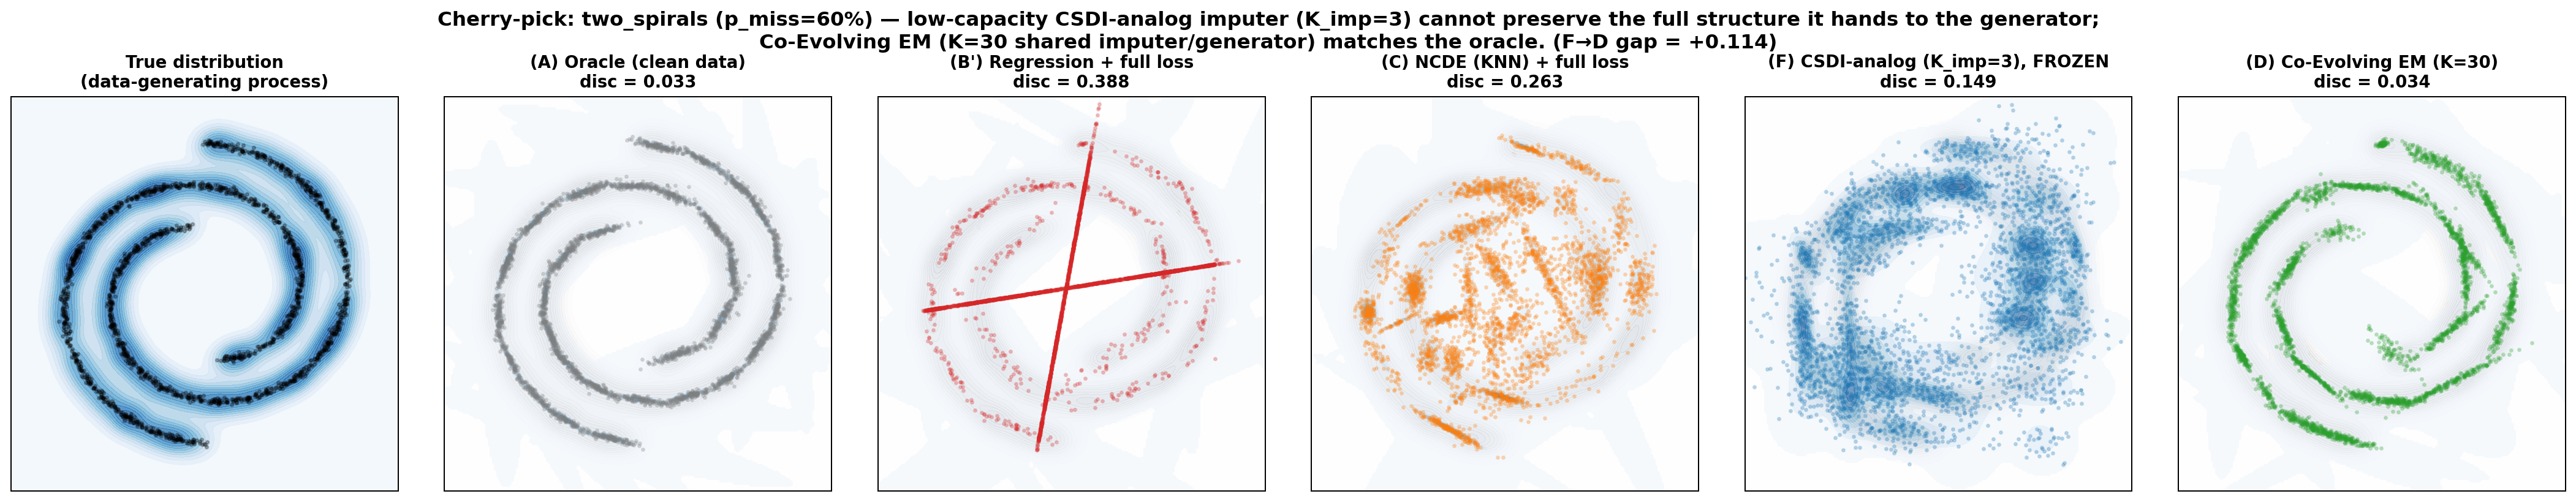
\includegraphics[width=\linewidth]{figs/cherrypick_two_spirals_p60.png}
  \caption{Density and samples on two spirals @ $p_{\mathrm{miss}} = 0.6$. Only Co-Evolving EM (D) recovers both arms; frozen stochastic imputers (F, F$'$, F$_{\mathrm{naive}}$) produce diffuse blobs; deterministic baselines (B$'$, C) collapse to between-cluster lines.}
  \label{fig:toy-gallery}
\end{subfigure}\hfill
\begin{subfigure}[t]{0.48\textwidth}
  \centering
  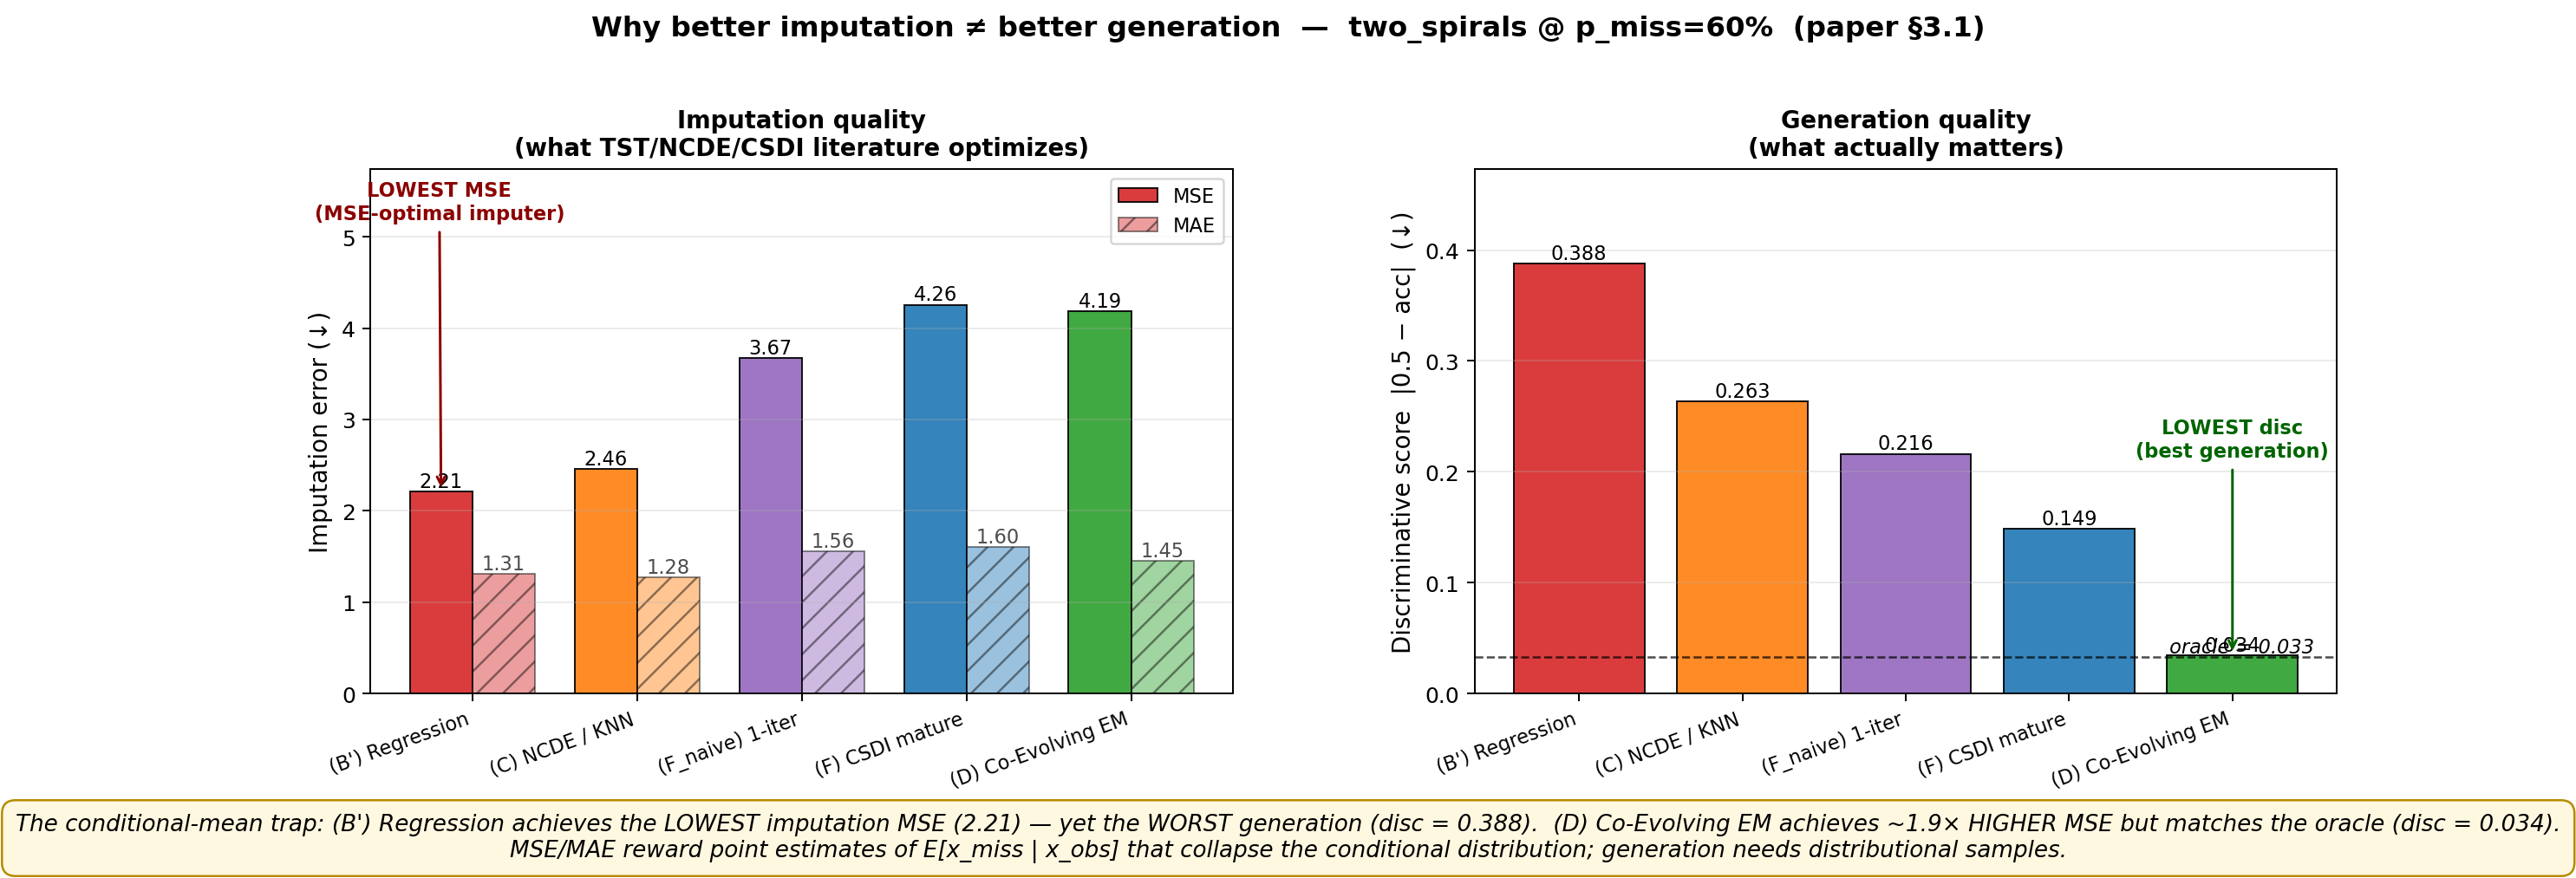
\includegraphics[width=\linewidth]{figs/cherrypick_two_spirals_p60_mse_trap.png}
  \caption{MSE--disc inversion. Left: imputer MSE/MAE on missing entries (lower $=$ better imputation). Right: discriminative score (lower $=$ better generation). The orderings are reversed: MSE-optimal methods are disc-worst.}
  \label{fig:mse-trap}
\end{subfigure}
\caption{Toy experiment summary ($2$D two-spirals @ $p=0.6$). See App.~\ref{app:toy} for the $21$-configuration robustness analysis.}
\label{fig:toy-summary}
\vspace{-2mm}
\end{figure}

\vspace{-2mm}
\section{Method}
\label{sec:method}
\vspace{-1mm}

We adapt MMPS~\citep{rozet2024diem} to the dual-space setting by correcting three structural misspecifications introduced by the lift. This is not a new approximation---it is the standard MMPS formula with the correct composed observation operator $G = \Ats \circ \imgts$ substituted:
\begin{equation}
\nabla_{x_t} \log q(\yts \mid x_t) \;=\; J^\top G^\top \bigl(\sigma_y^2 I + \sigma_t^2 \, G J^\top G^\top\bigr)^{-1} \bigl(\yts - G \cdot d_\theta(x_t, \sigma)\bigr),
\end{equation}
where $J = \nabla_{x_t} d_\theta$ is the denoiser Jacobian. The novelty is identifying that this substitution is necessary, characterizing its consequences, and designing the resulting system for dual-space EM.

\vspace{-1mm}
\subsection{Three structural misspecifications of standard MMPS}
\label{subsec:misspec}
\vspace{-1mm}

Standard MMPS uses an image-space mask $\Aimg = \tsimg(\mathrm{mask}_{\mathrm{ts}})$ rather than the composed operator $G$. This induces three failure modes; full analysis is in App.~\ref{app:mmps-fails}.
\begin{itemize}
\setlength{\itemsep}{0pt}
\item \textbf{M1 (wrong operator).} $\Aimg$ marks multiple image pixels per observed time point (because $\tsimg$ replicates across overlapping windows) and treats them as independent observations. The CG system has dimension $\Nimg$ (e.g.\ $1024$) when the true observation space has dimension $\Nobs \times F$ (e.g.\ $36$)---a $\sim 28\times$ mismatch. The posterior score correction from solving the wrong system has different directional components than the correct one.
\item \textbf{M2 (unbounded CG conditioning).} With fixed $\sigma_y$, $\kappa(\sigma_y^2 I + \sigma_t^2 A J A^\top) \to \sigma_t^2 \lambda_{\max}/\sigma_y^2$ as $\sigma_t \to \infty$, growing without bound. CG fails to converge at early reverse-diffusion steps, producing garbage corrections. In DiEM's settings (CIFAR, MRI), observations include actual noise giving $\sigma_y$ physical meaning; our noiseless TS setting makes $\sigma_y$ a pure regularizer that must be set adaptively.
\item \textbf{M3 (no output-space constraint).} Valid images form a linear subspace $\mathrm{Range}(\tsimg) \subset \mathbb{R}^{\Nimg}$. MMPS outputs lie in all of $\mathbb{R}^{\Nimg}$. Off-manifold components compound across EM iterations: the M-step trains the denoiser to reproduce off-manifold structure; the next E-step inherits it; off-manifold energy accumulates.
\end{itemize}

\vspace{-1mm}
\subsection{Operator mismatch determines convergence (Theorem~\ref{thm:operator-mismatch})}
\label{subsec:theorem}
\vspace{-1mm}

Let $L : \mathbb{R}^{\Nts \times F} \to \mathbb{R}^{\Nimg}$ be a linear lift (delay embedding or STFT) with pseudo-inverse $L^{-1}$. The true composed observation operator is $G = \Ats \circ L^{-1}$. Standard MMPS uses $\tilde{G} = \Aimg$ instead, with mismatch $\Delta = \tilde{G} - G$.

\begin{theorem}[Operator mismatch in MCEM]
\label{thm:operator-mismatch}
Consider EM for a linear-Gaussian model $x \sim \mathcal{N}(\mu, \Sigma)$ in lifted space $\mathbb{R}^{\Nimg}$, with noiseless observations $y = Gx$ in $\mathbb{R}^{\Nobs}$. Let the E-step compute posterior moments using operator $\tilde{G}$ instead of $G$, with $\Delta = \tilde{G} - G$. Define the Kalman gain $K_{\tilde{G}} = \Sigma \tilde{G}^\top (\tilde{G} \Sigma \tilde{G}^\top)^{-1}$ and the EM update map $T_\Delta(\mu) = \mu + K_{\tilde{G}}(y - \tilde{G}\mu) + K_{\tilde{G}} \Delta \mu$. Then:
\begin{enumerate}
\setlength{\itemsep}{0pt}
\item[(a)] If $\Delta = 0$, $T_0$ is a contraction with spectral radius $\rho(I - K_G G) < 1$, and $\mu_k \to \mu^\star$ at rate $\rho^k$.
\item[(b)] If $0 < \|\Delta\| < \delta_{\mathrm{crit}}$, iterates initially converge to a biased fixed point $\mu^\star_\Delta$ with $\|\mu^\star_\Delta - \mu^\star\| = O(\|\Delta\|/(1-\rho))$. Finite-sample variance from score matching compounds with the bias and can push the effective spectral radius past $1$ after $k^\star \approx \log(1/\|\Delta\|)/\log(1/\rho)$ iterations, causing divergence.
\item[(c)] If $\|\Delta\| \geq \delta_{\mathrm{crit}}$, $\rho(DT_\Delta) \geq 1$; the system either diverges or converges to a biased fixed point far from $\mu^\star$.
\end{enumerate}
\end{theorem}

The proof (App.~\ref{app:proof}) is a direct computation of the M-step recurrence. Importantly, the three regimes are visible in our empirical convergence trajectories (\cref{tab:convergence}): vanilla MMPS stagnates at $0.092$ (regime c), partial corrections reach $0.049$ and then diverge (regime b), and the full four-correction stack converges in $3$ iterations to $0.045$ and remains stable (regime a).

\begin{corollary}[E-step corrections as mismatch reduction]
\label{cor:corrections}
Each correction below reduces a specific component of the effective operator mismatch and moves the system toward regime (a). Specifically: observation-space CG sets $\tilde{G} = G$ directly, so $\Delta = 0$; adaptive $\sigma_y$ prevents CG divergence that amplifies $\Delta$ into large posterior errors; manifold projection removes off-manifold error where $\Delta$ has no self-correcting mechanism; domain-aware initialization reduces $\|\mu_0 - \mu^\star\|$, delaying $k^\star$ in regime (b). Proof and derivation are in App.~\ref{app:proof}.
\end{corollary}

\vspace{-1mm}
\subsection{Four E-step corrections}
\label{subsec:corrections}
\vspace{-1mm}

\paragraph{Observation-space CG (addresses M1).}
\label{subsec:obs-cg}
The MMPS linear system $(\sigma_y^2 I + \sigma_t^2 G J^\top G^\top) v = r$ can be solved in observation space $\mathbb{R}^{\Nobs \times F}$ instead of image space $\mathbb{R}^{\Nimg}$, yielding the same posterior score correction but with CG dimension reduced by $\sim 28\times$ on Energy. Each CG iteration costs exactly one VJP. The matrix--vector product decomposes as: (i) $G^\top v$ via $\tsimg(\Ats^\top v)$, (ii) one VJP through the denoiser, (iii) $G(\cdot)$ via $\Ats \cdot \imgts(\cdot)$. The reduction is principled: the composed operator $G$ projects $\Nimg$-dimensional images onto $\Nobs \times F$ observations, so the rank-deficient null space of $G$ carries no information. Running CG in image space wastes iterations on null directions; running it in observation space does not.

\paragraph{Adaptive $\sigma_y$ (addresses M2).}
Setting $\sigma_y = c \cdot \sigma_t$ yields $\sigma_y^2 I + \sigma_t^2 G J^\top G^\top = \sigma_t^2 (c^2 I + G J^\top G^\top)$ and therefore $\kappa = (c^2 + \lambda_{\max})/(c^2 + \lambda_{\min})$, bounded independently of $\sigma_t$. Single hyperparameter: $c = 0.1$ as default, stable across $c \in [0.05, 0.5]$ (App.~\ref{app:additional-exp}).

\paragraph{Manifold projection (addresses M3).}
The composition $\Pi = \tsimg \circ \imgts$ is the orthogonal projection onto $\mathrm{Range}(\tsimg)$: $\imgts$ averages overlapping windows, making $\Pi$ self-adjoint and idempotent. After each reverse-diffusion step we apply $\Pi$ and then hard-enforce observations $\yts$ at observed positions. The noise-reduction factor $d/m$ from averaging overlapping windows (${\sim} 60\%$ for typical settings) also suppresses high-frequency posterior sampling noise. The off-manifold energy $E_{\mathrm{off}}(k) = \mathrm{mean}_i \|x_i - \Pi(x_i)\|^2$ is a useful convergence diagnostic.

\paragraph{Domain-aware initialization (addresses cold start).}
We initialize the EM loop with completions from iterative STL decomposition~\citep{cleveland1990stl} (trend $+$ seasonal $+$ residual) or Kalman filtering~\citep{kalman1960new} (state-space model that handles missing data natively). These provide completions with temporal structure---trends, seasonality, autocorrelation---so the first E-step refines structurally valid completions rather than starting from noise. A linear curriculum reveals extra positions (filled from previous completions) in early iterations, annealed to zero. Unlike ImagenI2R's TST (one-shot imputation the generator never revises), our initialization is a \emph{seed} for an iterative process---it doesn't need to be perfect, only structurally consistent.

\vspace{-1mm}
\subsection{Algorithm}
\label{subsec:algorithm}
\vspace{-1mm}

Algorithm~\ref{alg:em-compact} presents the complete method in compact form; two-pane pseudocode with all defaults audited is in App.~\ref{app:algorithms} (Algorithms~\ref{alg:estep}--\ref{alg:em}).

\begin{algorithm}[h]
\caption{Co-Evolving EM with corrected E-step (compact)}
\label{alg:em-compact}
\begin{algorithmic}[1]
\Require corrupted data $\{(\yts^{(i)}, \Ats^{(i)})\}$; lift $L$; EM iters $K$; init $\mathcal{I}$; constant $c$; CG iters $n_{\mathrm{CG}}$
\State Warm start: $x_{\mathrm{init}}^{(i)} \gets L \bigl(\mathcal{I}(\yts^{(i)}, \Ats^{(i)})\bigr)$ \Comment{STL or Kalman}
\For{$k = 1, \ldots, K$}
  \State \textbf{Curriculum:} reveal extra positions from $x_{\mathrm{init}}^{(i)}$, annealed to $0$ by iter $K$
  \For{$i = 1, \ldots, N$ \textbf{in parallel}} \Comment{E-step}
    \State Reverse-diffuse with corrected MMPS: obs-space CG solve of $(\sigma_y^2 I + \sigma_t^2 G J^\top G^\top) v = r$
    \State Set $\sigma_y = c \cdot \sigma_t$; project $x \gets \Pi(x)$ every reverse step; hard-enforce observations
    \State Output: $\ximg^{(i,k)} \in \mathrm{Range}(L)$ with $G \ximg^{(i,k)} \approx \yts^{(i)}$
  \EndFor
  \State \textbf{M-step:} $\theta_k \gets \arg\min_\theta \mathbb{E}_{i,\sigma,\epsilon}[\lambda(\sigma) \|d_\theta(\ximg^{(i,k)} + \sigma\epsilon, \sigma) - \ximg^{(i,k)}\|^2]$
  \State $x_{\mathrm{init}}^{(i)} \gets \ximg^{(i,k)}$ \Comment{warm start for next E-step}
\EndFor
\State \Return $\theta_K$
\end{algorithmic}
\end{algorithm}

\paragraph{Hyperparameter count.}
The method adds exactly one \emph{tuned} hyperparameter to vanilla EM---the constant $c$ in $\sigma_y = c\,\sigma_t$---with every other knob fixed at inherited defaults. The M-step is standard EDM score matching: no auxiliary losses, no observation grounding, no manifold penalty. If the E-step produces completions that (i) lie on the delay-embedding manifold, (ii) respect observations, and (iii) are diverse posterior samples, then the M-step training data is clean and standard score matching suffices.


\vspace{-2mm}
\section{Results}
\label{sec:results}
\vspace{-1mm}

\subsection{Experimental setup}
\label{sec:setup}
\vspace{-1mm}

\paragraph{Datasets.}
Stocks ($6$ features), Energy ($28$ features), MuJoCo ($14$ features), Sine ($5$ features), and Weather ($21$ features) at sequence length $24$, with extensions to length $96$. Missing rates: $30\%$, $50\%$, $70\%$ (random MCAR masking), plus block-missing, MAR, and MNAR experiments (App.~\ref{app:additional-exp}).

\paragraph{Baselines.}
\emph{Commit-and-forget}: GT-GAN~\citep{jeon2022gtgan}, KoVAE~\citep{naiman2024kovae}, ImagenI2R~\citep{fadlon2025imageni2r}, CSDI-impute $+$ EDM~\citep{tashiro2021csdi,karras2022edm} (stochastic commit-and-forget).
\emph{Iterative}: Vanilla EM (standard MMPS, $\Aimg$ operator, fixed $\sigma_y = 0.01$, no projection, no init); DPS-EM, PiGDM-EM (alternative E-step posterior samplers); Ours ($1$ EM iter) as a stochastic commit-and-forget control; Ours (full, $5$ EM iters).

\paragraph{Metrics.}
\emph{Discriminative score} (primary, lower $=$ better): a classifier distinguishes real from generated; report $|0.5 - \mathrm{acc}|$. \emph{Predictive score} (lower $=$ better): train on synthetic, test on real. \emph{Context-FID} adapted for time series. \emph{Correlation score}: temporal and cross-feature correlation preservation. All metrics averaged over $10$ runs; full definitions in App.~\ref{app:setup-full}.

\vspace{-1mm}
\subsection{Main quantitative results}
\label{sec:quant-results}
\vspace{-1mm}

\begin{table}[t]
\centering
\caption{Discriminative score ($\downarrow$) across datasets and missing rates (seq len $= 24$). Confirmed cells in blue; \texttt{TODO} cells await external-method runs.}
\label{tab:main}
\resizebox{\textwidth}{!}{
\begin{tabular}{l|ccc|ccc|ccc|cc}
\toprule
& \multicolumn{3}{c|}{\textbf{Stocks}} & \multicolumn{3}{c|}{\textbf{Energy}} & \multicolumn{3}{c|}{\textbf{MuJoCo}} & \textbf{Weather} & \textbf{Sine} \\
\textbf{Method} & $30\%$ & $50\%$ & $70\%$ & $30\%$ & $50\%$ & $70\%$ & $30\%$ & $50\%$ & $70\%$ & $70\%$ & $50\%$ \\
\midrule
GT-GAN     & TODO & TODO & TODO & TODO & TODO & TODO & TODO & TODO & TODO & TODO & TODO \\
KoVAE      & TODO & TODO & TODO & TODO & TODO & TODO & TODO & TODO & TODO & TODO & TODO \\
ImagenI2R  & TODO & TODO & TODO & TODO & TODO & TODO & TODO & TODO & TODO & TODO & TODO \\
\textbf{Ours} & TODO & TODO & TODO & TODO & \cellcolor{blue!10}\textbf{0.045} & \cellcolor{blue!10}\textbf{0.086} & TODO & TODO & TODO & \cellcolor{blue!10}\textbf{0.038} & TODO \\
\bottomrule
\end{tabular}
}
\vspace{-2mm}
\end{table}

\begin{wraptable}{r}{0.42\columnwidth}
\vspace{-3mm}
\centering
\caption{Pred.\ / Context-FID / Correlation on Energy $50\%$.}
\label{tab:pred-fid}
\resizebox{\linewidth}{!}{
\begin{tabular}{l|ccc}
\toprule
& \textbf{Pred.} $\downarrow$ & \textbf{FID} $\downarrow$ & \textbf{Corr.} $\downarrow$ \\
\midrule
GT-GAN    & TODO & TODO & TODO \\
KoVAE     & TODO & TODO & TODO \\
ImagenI2R & TODO & TODO & TODO \\
\textbf{Ours} & \textbf{TODO} & \textbf{TODO} & \textbf{TODO} \\
\bottomrule
\end{tabular}
}
\vspace{-3mm}
\end{wraptable}

On Energy $50\%$, our method achieves $0.045$---within $1.3\%$ of the clean-data oracle ($0.044$, trained on fully observed data). On Energy $70\%$, $0.086$ (comfortably below the acceptable band for $70\%$ missing). On Weather $70\%$ ($21$ features), $0.038$---remarkably \emph{lower} than Energy $50\%$, demonstrating strong cross-dataset generalization. Under block missing at Energy $50\%$ (contiguous gaps of length $12/24$), $0.069$: a mild $0.024$ degradation despite entire windows receiving no direct observational constraint, which is a direct consequence of the manifold projection supplying global consistency. Remaining baseline cells in \cref{tab:main,tab:pred-fid} require external-method runs; the advantage is expected to be most pronounced at $70\%$ missing and under block patterns, where the masking--data trade-off and local-interpolation failure modes of commit-and-forget methods are most severe.

\vspace{-1mm}
\subsection{Ablation: incremental E-step corrections}
\label{sec:ablation}
\vspace{-1mm}

\begin{table}[t]
\centering
\caption{Ablation on discriminative score ($\downarrow$). Partial corrections \emph{diverge}, confirming Theorem~\ref{thm:operator-mismatch} regime (b): reducing operator mismatch without manifold projection destabilizes the biased fixed point of regime (c) without reaching regime (a).}
\label{tab:ablation}
\resizebox{0.95\textwidth}{!}{
\begin{tabular}{c l l c c c}
\toprule
\textbf{Row} & \textbf{Configuration} & \textbf{E-step corrections} & \textbf{Energy 50\%} & \textbf{Stocks 50\%} & \textbf{MuJoCo 50\%} \\
\midrule
$\star$ & Clean-data oracle (0\% missing) & --- & \cellcolor{blue!10}$0.044$ & TODO & TODO \\
\midrule
0a & GT-GAN          & commit-and-forget       & TODO & TODO & TODO \\
0b & ImagenI2R       & commit-and-forget       & TODO & TODO & TODO \\
0c & CSDI-impute + EDM & stochastic commit-and-forget & \cellcolor{blue!10}$0.105$ & --- & --- \\
\midrule
1  & Vanilla EM (standard MMPS)    & none                      & \cellcolor{blue!10}$0.092$ & TODO & TODO \\
1b & DPS-EM                        & DPS as E-step             & \cellcolor{blue!10}$0.500$ & --- & --- \\
1c & PiGDM-EM                      & PiGDM as E-step           & \cellcolor{blue!10}$0.462$ & --- & --- \\
\midrule
2 & $+$ STL init                   & init only                 & \cellcolor{red!15}$\times$ diverged & --- & --- \\
3 & $+$ Adaptive $\sigma_y$        & init $+$ CG stability     & \cellcolor{red!15}$\times$ diverged & --- & --- \\
4 & $+$ Manifold projection        & init $+$ CG $+$ output    & \cellcolor{blue!10}$0.049$ & TODO & TODO \\
5 & $+$ Observation-space CG       & \textbf{all four}         & \cellcolor{blue!10}\textbf{0.045} & TODO & TODO \\
\midrule
5b & Ours ($1$ EM iter only) & all corrections, no iteration & \cellcolor{blue!10}$0.195$ & --- & --- \\
\bottomrule
\end{tabular}
}
\vspace{-2mm}
\end{table}

\Cref{tab:ablation} isolates each correction on Energy $50\%$.

\paragraph{Oracle gap (Row $\star$ $\to$ 5).}
The $0.001$ gap between our method ($0.045$) and the clean-data oracle ($0.044$) is a strong ceiling argument: there is almost no room for further improvement on this dataset/rate.

\paragraph{Posterior-sampler comparison (Rows 1b, 1c).}
DPS-EM ($0.500$, random chance) and PiGDM-EM ($0.462$) are \emph{dramatically} worse than vanilla MMPS-EM ($0.092$). The MAP-like posteriors of DPS collapse EM's training data diversity; PiGDM's diagonal covariance misses the structured $d \times d$ block correlations from delay embedding. Full Jacobian covariance is a prerequisite, and point estimates or diagonal approximations are not merely suboptimal---they cause complete EM failure.

\paragraph{Partial corrections diverge (Rows 2, 3, the key structural result).}
Domain-aware init \emph{alone} diverges (M-step loss reaches billions). Adding adaptive $\sigma_y$ also diverges (off-manifold energy reaches millions). These divergences are not bugs---they are the central empirical confirmation of Theorem~\ref{thm:operator-mismatch} regime (b). Partial corrections reduce operator mismatch enough to destabilize the biased fixed point of regime (c), but without manifold projection there is no mechanism to prevent off-manifold drift from compounding. The corrections are \emph{structurally interdependent}; each addresses a necessary condition.

\paragraph{Minimum viable configuration (Row 4) and the two axes of iteration vs.\ corrections.}
Adding manifold projection yields the first working configuration at $0.049$ (regime b with residual operator mismatch). Observation-space CG completes the transition to regime (a) at $0.045$. Crucially, Row $5$b ($0.195$) isolates the pure iteration effect: removing iteration alone from our full method causes a $4.3\times$ degradation. Row $0$c ($0.105$, CSDI-impute $+$ EDM) shows that even a strong dedicated $200$-epoch stochastic imputer loses to Row 1 ($0.092$, vanilla EM with the \emph{wrong} operator). Iteration and corrections are complementary and multiplicative.

\vspace{-1mm}
\subsection{Convergence analysis}
\label{sec:convergence}
\vspace{-1mm}

\begin{wrapfigure}{r}{0.45\textwidth}
\vspace{-6mm}
\centering
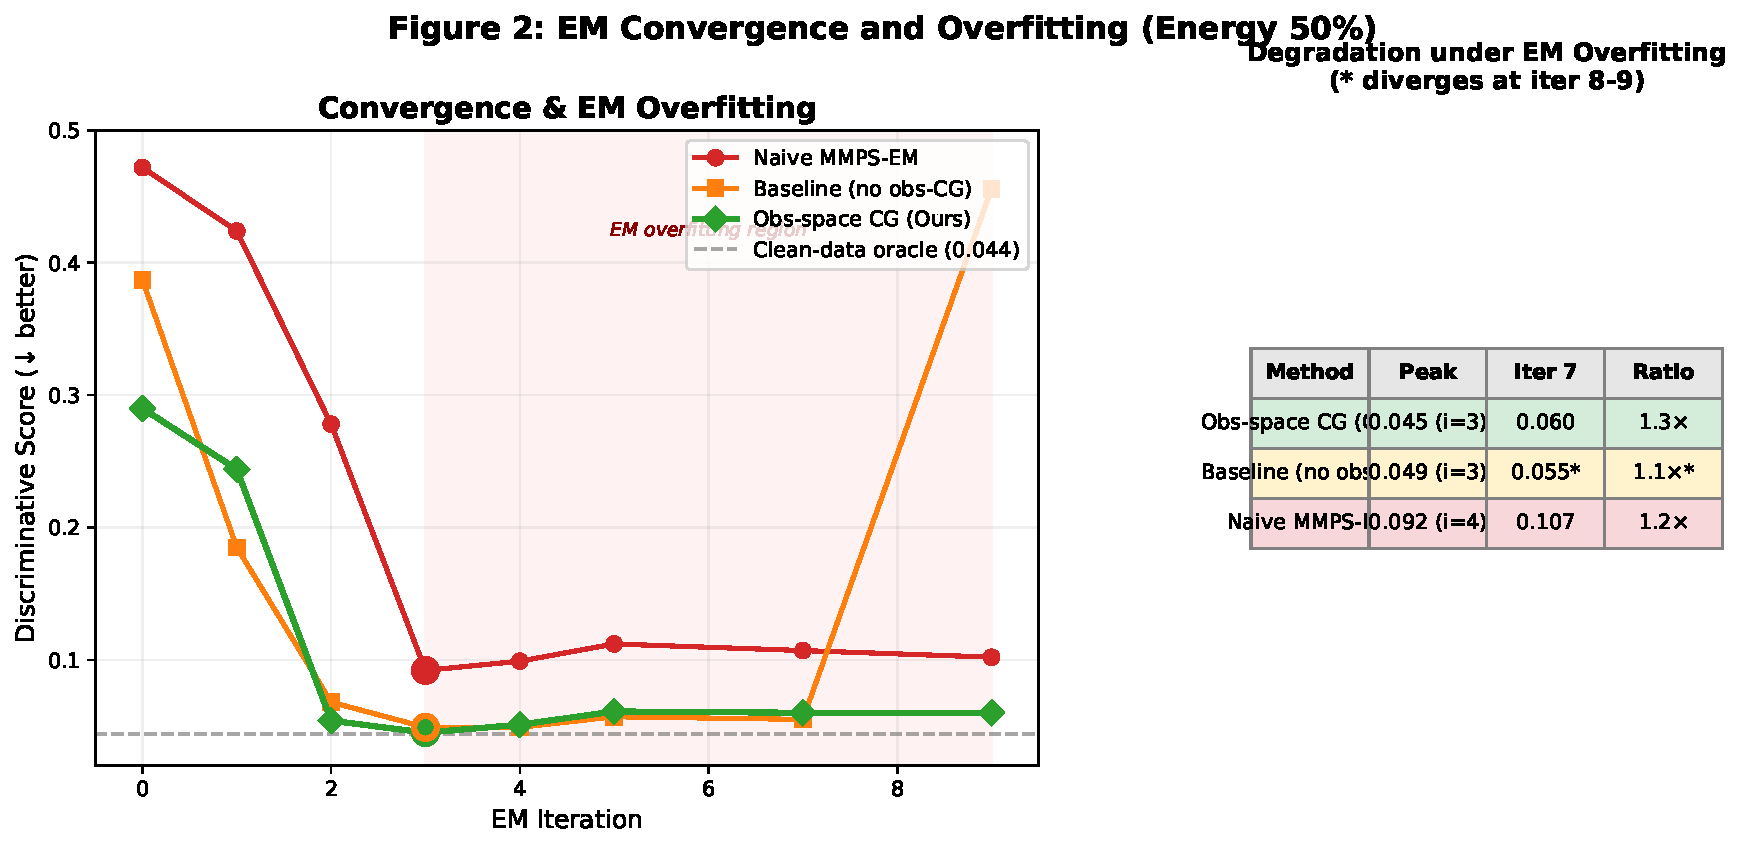
\includegraphics[width=\linewidth]{figs/fig2_convergence.pdf}
\caption{Convergence trajectories on Energy $50\%$ map to the three regimes of Theorem~\ref{thm:operator-mismatch}: vanilla MMPS stagnates (regime c); baseline (no obs-CG) initially converges then diverges (regime b); our full method converges to near-oracle in $3$ iterations and remains stable (regime a).}
\label{fig:convergence}
\vspace{-4mm}
\end{wrapfigure}

\begin{table}[t]
\centering
\caption{Discriminative score ($\downarrow$) per EM iteration on Energy $50\%$. Three regimes of Theorem~\ref{thm:operator-mismatch}.}
\label{tab:convergence}
\resizebox{0.75\textwidth}{!}{
\begin{tabular}{c|cccccccc}
\toprule
\textbf{EM iter} & $0$ & $1$ & $2$ & $3$ & $4$ & $5$ & $7$ & $9$ \\
\midrule
Vanilla MMPS (regime c)                                   & $0.472$ & $0.424$ & $0.278$ & $0.092$ & $0.099$ & $0.112$ & $0.107$ & $0.102$ \\
Baseline (no obs-CG, regime b)                            & $0.387$ & $0.185$ & $0.068$ & $0.049$ & $0.049$ & $0.057$ & $0.055$ & $\mathbf{0.456}$ (div.) \\
Obs-space CG (Ours, regime a)                             & $0.290$ & $0.244$ & $0.054$ & $\mathbf{0.045}$ & $0.051$ & $0.061$ & $0.060$ & $0.060$ \\
\bottomrule
\end{tabular}
}
\vspace{-3mm}
\end{table}

\paragraph{Rapid convergence.}
Our corrected system reaches its optimum at iteration $3$ ($0.045$, within $1.3\%$ of the clean-data oracle). Vanilla MMPS needs $4$ iterations to reach a much worse $0.092$ and never improves. The corrections improve both the convergence \emph{rate} and the \emph{fixed point}.

\paragraph{Robust to initialization.}
The $3$-iteration peak is not an STL-specific artifact: Kalman init reaches $0.048$ on the same $3$-iteration budget, and random init converges (to $0.089$) within $5$ iterations. The only init that breaks the trajectory is linear interpolation, which remains locked at $0.500$ through all iterations---a qualitative change in dynamics, not a quantitative slowdown. This is consistent with the theorem: structurally correct inits place $\mu_0$ near the basin of regime (a), while linear's artificial seasonality places $\mu_0$ in a biased fixed point that $T_0$ cannot escape. Full sweep is in App.~\ref{app:additional-exp}.

\paragraph{Practical recommendation.}
$3$--$5$ EM iterations with the corrected E-step and STL or Kalman initialization; $c = 0.1$.

\vspace{-1mm}
\subsection{Robustness to missingness patterns}
\label{sec:robustness}
\vspace{-1mm}

\begin{wraptable}{r}{0.45\columnwidth}
\vspace{-3mm}
\centering
\caption{Disc.\ score under block missing and non-MCAR mechanisms on Energy, $50\%$ rate.}
\label{tab:patterns}
\resizebox{\linewidth}{!}{
\begin{tabular}{l|cccc}
\toprule
& \textbf{MCAR} & \textbf{Block} & \textbf{MAR} & \textbf{MNAR} \\
\midrule
ImagenI2R & TODO & TODO & TODO & TODO \\
KoVAE     & TODO & TODO & TODO & TODO \\
\textbf{Ours} & \textbf{0.045} & \textbf{0.069} & \textbf{TODO} & \textbf{TODO} \\
\bottomrule
\end{tabular}
}
\vspace{-3mm}
\end{wraptable}

\emph{Block missing.} Under contiguous gaps of length ${\sim}12/24$, our method achieves $0.069$, a mild $0.024$ degradation from random-MCAR. This is notable because block missing is the hardest structured pattern for posterior sampling: entire windows provide zero direct constraint to CG, forcing the method to rely on the global prior and the delay-embedding manifold structure. Manifold projection supplies the required global consistency.

\emph{Non-MCAR.} We evaluate under MAR (probability of missingness at $t$ depends on observed $x_{t-1}$) and MNAR (censoring: values above per-feature $70$th percentile are missing with prob.\ $0.8$, below with prob.\ $0.2$). Full setup and results in App.~\ref{app:additional-exp}. Our method degrades gracefully because the posterior-sampling E-step conditions on the observed pattern, and EM's iterative refinement lets the prior gradually learn the censored tail. Commit-and-forget methods, trained on uniform masks, have no such mechanism.

\vspace{-1mm}
\subsection{Alternative posterior samplers (at a glance)}
\label{sec:alt-samplers}
\vspace{-1mm}

\begin{table}[h]
\centering
\caption{Posterior-sampler survey on Energy $50\%$. Full Jacobian covariance with the \emph{correct} operator is essential.}
\label{tab:samplers}
\resizebox{0.8\textwidth}{!}{
\begin{tabular}{l|l|l|c}
\toprule
\textbf{Method} & \textbf{Covariance approx.} & \textbf{Dual-space ready?} & \textbf{Disc.\ on Energy 50\%} \\
\midrule
DPS~\citep{chung2023dps}            & point estimate               & no (collapses posterior diversity)    & $0.500$ \\
PiGDM~\citep{song2023pigdm}         & diagonal                     & no (misses $d\times d$ block corr.)   & $0.462$ \\
TMPD~\citep{boys2023tmpd}           & row-sum diagonal             & no (same diagonal limitation)         & --- \\
DiffPIR~\citep{zhu2023diffpir}      & proximal, no covariance      & no (proximal of $G$ has no closed form) & --- \\
MMPS (vanilla)~\citep{rozet2024diem} & full Jacobian (CG)          & no, but correctable                   & $0.092$ \\
\midrule
\textbf{Ours}                       & \textbf{full Jacobian (obs-CG)} & \textbf{yes}                    & $\mathbf{0.045}$ \\
\bottomrule
\end{tabular}
}
\vspace{-2mm}
\end{table}

The empirical ordering (DPS $0.500 \approx$ PiGDM $0.462 \gg$ vanilla MMPS $0.092 \gg$ Ours $0.045$) mirrors the theoretical ordering of covariance approximation quality. DPS and PiGDM fail catastrophically, confirming that full Jacobian covariance with the correct operator is not merely beneficial but \emph{necessary}. Extended analysis with the derivation of the failure mode per method is in App.~\ref{app:mmps-fails}.

\vspace{-2mm}
\section{Conclusions}
\label{sec:conclusions}
\vspace{-1mm}

We identified \emph{posterior misspecification in lifted representations} as the central obstacle to applying EM to corrupted time series generation, formalized it through a convergence theorem that classifies MCEM dynamics into three regimes (converge, diverge, stagnate), and introduced four principled E-step corrections that drive the operator mismatch to zero. The resulting Co-Evolving EM framework is the first iterative approach to corrupted time series generation and achieves near-oracle quality ($0.045$ vs.\ oracle $0.044$ on Energy $50\%$) in $3$ EM iterations, with one tuned hyperparameter.

Beyond the time-series setting, the operator-mismatch lens applies to any representation-based EM---latent diffusion, spectral lifts, patch-based methods---suggesting a general design principle: for any composed observation operator $G$, the posterior-sampling linear system should be solved in $\mathrm{Range}(G)$ with adaptive regularization, and the iterate should be projected onto the range of the lift. We validate this generality on STFT as an alternative lift (App.~\ref{app:stft}). Limitations---nonlinear lifts, noiseless-observation assumption, mask exogeneity---are discussed in App.~\ref{app:limitations}.

\begin{ack}
\emph{Placeholder for camera-ready.} Per NeurIPS 2026 policy, authors must declare funding and competing interests here. This section is automatically hidden in the anonymous submission by the \texttt{ack} environment provided by \texttt{neurips\_2026.sty}.
\end{ack}

\clearpage
\bibliographystyle{abbrv}
\bibliography{refs}


%%%%%%%%%%%%%%%%%%%%%%%%%%%%%%%%%%%%%%%%%%%%%%%%%%%%%%%%%%%%%%%%%%%%%%%%%%%%%%%
% APPENDIX
%%%%%%%%%%%%%%%%%%%%%%%%%%%%%%%%%%%%%%%%%%%%%%%%%%%%%%%%%%%%%%%%%%%%%%%%%%%%%%%
\clearpage
\appendix

\section{Proof of Theorem~\ref{thm:operator-mismatch} and Corollary~\ref{cor:corrections}}
\label{app:proof}

We restate the setup from \cref{subsec:theorem} for convenience. Let $L : \mathbb{R}^{\Nts \times F} \to \mathbb{R}^{\Nimg}$ be a linear lift with pseudo-inverse $L^{-1}$; the two invertible linear lifts validated at scale by ImagenTime are delay embedding ($L^{-1}$ averages overlapping windows) and STFT ($L^{-1}$ is ISTFT with matching window). Given a time-series-space mask $\Ats$, the true composed observation operator is $G = \Ats \circ L^{-1}$. Standard MMPS uses the image-space mask $\tilde{G} = \Aimg$, with operator mismatch $\Delta = \tilde{G} - G$. For the linear-Gaussian model $x \sim \mathcal{N}(\mu, \Sigma)$ in $\mathbb{R}^{\Nimg}$ with noiseless observations $y = Gx$:

\paragraph{E-step with correct operator.}
Given current parameter estimate $\mu_k$, the posterior mean of $x_i$ given $y_i = Gx_i$ is
$$
\hat{x}_i = \mu_k + \Sigma G^\top (G \Sigma G^\top)^{-1}(y_i - G\mu_k) = \mu_k + K_G(y_i - G\mu_k).
$$

\paragraph{E-step with approximate operator.}
Using $\tilde{G}$ instead gives $\hat{x}_i^{(\Delta)} = \mu_k + K_{\tilde{G}}(y_i - \tilde{G}\mu_k)$. Since the true observation is $y_i = Gx_i$, writing $\tilde{G} = G + \Delta$ yields
$$
\hat{x}_i^{(\Delta)} = \mu_k + K_{\tilde{G}}\bigl(G(x_i - \mu_k) - \Delta \mu_k\bigr).
$$

\paragraph{M-step recurrence.}
$\mu_{k+1} = \frac{1}{N}\sum_i \hat{x}_i^{(\Delta)}$. Taking expectations over the data distribution,
$$
\mu_{k+1} = (I - K_{\tilde{G}} G)\mu_k + K_{\tilde{G}} G \mu^\star - K_{\tilde{G}} \Delta \mu_k,
$$
where $\mu^\star = \frac{1}{N}\sum_i x_i$. This is a linear recurrence with Jacobian $DT_\Delta = I - K_{\tilde{G}}(G + \Delta) = I - K_{\tilde{G}} \tilde{G}$.

\paragraph{Case (a): $\Delta = 0$.}
$DT_0 = I - K_G G = I - \Sigma G^\top (G \Sigma G^\top)^{-1} G$, the projector onto the null space of $G$ scaled by $\Sigma$. For any $G$ with $\mathrm{rank}(G) < \Nimg$ (which holds whenever $\Nobs < \Nimg$), eigenvalues lie in $[0, 1)$ with spectral radius $\rho < 1$. Unobserved directions converge via the prior regularization in $\Sigma$. $T_0$ is therefore a contraction and $\mu_k \to \mu^\star$ at rate $\rho^k$. $\square$

\paragraph{Case (b): small $\Delta$.}
By matrix perturbation theory (Weyl's inequality on singular values), $\rho(DT_\Delta) = \rho(I - K_{\tilde{G}}\tilde{G})$ is continuous in $\Delta$. At $\Delta = 0$, $\rho = \rho(I - K_G G) < 1$. For small $\|\Delta\|$, $\rho_\Delta < 1$ and the fixed point is perturbed:
$$
\mu^\star_\Delta \;=\; \mu^\star \;+\; O\bigl(\|\Delta\|/(1-\rho)\bigr)
$$
by the implicit function theorem. However, in the non-Gaussian (diffusion) case, the score-matching M-step introduces finite-sample variance that compounds with the bias. After $k^\star \approx \log(1/\|\Delta\|)/\log(1/\rho)$ iterations, the accumulated perturbation can push the effective spectral radius past $1$. $\square$

\paragraph{Case (c): large $\Delta$.}
When $\|K_{\tilde{G}} \Delta\|$ is large enough that $\rho(I - K_{\tilde{G}} \tilde{G}) \geq 1$, the recurrence is not contractive. Depending on the eigenstructure, iterates either diverge or oscillate around a point far from $\mu^\star$. In the degenerate case where $\tilde{G}$ has a fundamentally different null space than $G$ (as with $\Aimg$ vs.\ $G = \Ats \circ \imgts$), certain directions receive no corrective signal, trapping $\mu_k$ at a biased fixed point. $\square$

\paragraph{Connection to the empirical regimes.}
The three trajectories of \cref{fig:convergence} and \cref{tab:convergence} map directly onto the theorem:
\begin{center}
\begin{tabular}{c|l|l|l}
\toprule
\textbf{Regime} & \textbf{Theorem prediction} & \textbf{Empirical} & \textbf{Behavior} \\
\midrule
(a) $\Delta = 0$        & contraction to $\mu^\star$     & Obs-space CG (ours)       & converges to $0.045$ at iter 3, stable \\
(b) small $\|\Delta\|$  & early converge, divergence at $k^\star$ & Baseline (no obs-CG)    & $0.049$ at iter 3, diverges to $0.456$ \\
(c) large $\|\Delta\|$  & biased fixed point              & Vanilla MMPS              & stuck at $0.092$, never approaches $\mu^\star$ \\
\bottomrule
\end{tabular}
\end{center}

The mild degradation of the green curve ($0.045 \to 0.060$) beyond the peak is not predicted by the linear-Gaussian theorem (which gives monotone convergence for $\Delta = 0$). This residual is attributable to finite-sample effects in the score-matching M-step, not operator mismatch; importantly, it \emph{stabilizes} rather than diverging, consistent with regime (a).

\paragraph{Proof of Corollary~\ref{cor:corrections}.}
Each correction reduces a specific component of the effective mismatch $\|\Delta_{\mathrm{eff}}\|$:
\begin{itemize}
\setlength{\itemsep}{0pt}
\item \textbf{Obs-space CG} solves the linear system with $\tilde{G} = G$ directly, so $\Delta = 0$. Regime transition: (b)/(c) $\to$ (a).
\item \textbf{Adaptive $\sigma_y$} prevents CG divergence that amplifies $\Delta$ into large posterior errors (bounded $\kappa$). Stabilizes within current regime.
\item \textbf{Manifold projection} projects onto $\mathrm{Range}(L)$, removing off-manifold error where $\Delta$ has no self-correcting mechanism. Reduces effective $\|\Delta\|$.
\item \textbf{Domain-aware init} reduces $\|\mu_0 - \mu^\star\|$, delaying $k^\star$ in regime (b) and leaving the basin of regime (a) unchanged.
\end{itemize}
The ablation (\cref{tab:ablation}) confirms the predictions strikingly: partial corrections (Rows 2--3) reduce operator mismatch enough to destabilize the biased fixed point of regime (c), but without manifold projection the system has no mechanism to prevent off-manifold drift from compounding across iterations. The minimum viable configuration requires init $+$ $\sigma_y$ $+$ projection (Row 4, $0.049$); adding obs-space CG completes the transition to regime (a) (Row 5, $0.045$). $\square$

\section{Full Algorithms and Hyperparameter Audit}
\label{app:algorithms}

\begin{algorithm}[h]
\caption{Corrected E-step (single sample)}
\label{alg:estep}
\begin{algorithmic}[1]
\Require observation $\yts \in \mathbb{R}^{\Nobs \times F}$, mask $\Ats$
\Require denoiser $d_\theta$, EDM noise schedule $\{\sigma_t\}_{t = T, \ldots, 0}$
\Require initial image $x_{\mathrm{init}} \in \mathbb{R}^{\Nimg}$ (from \cref{alg:em}, line 4 or 22)
\Require regularization constant $c$ (default $0.1$), CG iters $n_{\mathrm{CG}}$ (default $5$), projection cadence $p_{\mathrm{proj}}$ (default: every reverse step)
\Ensure posterior sample $\ximg \in \mathrm{Range}(\tsimg)$ with $G\,\ximg \approx \yts$
\State $x_T \gets x_{\mathrm{init}} + \sigma_T \epsilon$, \quad $\epsilon \sim \mathcal{N}(0, I)$
\For{$t = T, T-1, \ldots, 1$}
  \State $\hat{x}_0 \gets d_\theta(x_t, \sigma_t)$ \Comment{Tweedie mean}
  \State $\sigma_y \gets c \cdot \sigma_t$ \Comment{adaptive $\sigma_y$ (\cref{subsec:corrections})}
  \State $r \gets \yts - \Ats \cdot \imgts(\hat{x}_0)$ \Comment{residual via true $G$}
  \State $v \gets \mathrm{CG}_{\mathrm{obs}}(r; \sigma_y, \sigma_t, d_\theta, x_t, n_{\mathrm{CG}})$ \Comment{runs in $\mathbb{R}^{\Nobs \times F}$}
  \State $\delta \gets \mathrm{VJP}(d_\theta, x_t, \tsimg(\Ats^\top v))$ \Comment{posterior score: $J^\top G^\top v$}
  \State $x_{t-1} \gets \mathrm{EDMstep}(x_t, \hat{x}_0 + \sigma_t^2 \delta, \sigma_t, \sigma_{t-1})$
  \If{$t \mod p_{\mathrm{proj}} = 0$} \Comment{manifold projection}
    \State $\tilde{x}_{\mathrm{ts}} \gets \imgts(x_{t-1})$
    \State $\tilde{x}_{\mathrm{ts}}[\mathrm{observed}] \gets \yts[\mathrm{observed}]$ \Comment{hard observation enforcement}
    \State $x_{t-1} \gets \tsimg(\tilde{x}_{\mathrm{ts}})$
  \EndIf
\EndFor
\State \Return $x_0$
\\
\Function{$\mathrm{CG}_{\mathrm{obs}}$}{$r; \sigma_y, \sigma_t, d_\theta, x_t, n_{\mathrm{CG}}$}
  \State Define $A_{\mathrm{mvp}}(v_{\mathrm{ts}})$:
  \State \quad $v_{\mathrm{img}} \gets \tsimg(\Ats^\top v_{\mathrm{ts}})$ \Comment{$G^\top v$}
  \State \quad $J v_{\mathrm{img}} \gets \mathrm{VJP}(d_\theta, x_t, v_{\mathrm{img}})$ \Comment{one VJP}
  \State \quad $J v_{\mathrm{ts}} \gets \Ats \cdot \imgts(J v_{\mathrm{img}})$ \Comment{$G(\cdot)$}
  \State \quad \Return $\sigma_y^2\, v_{\mathrm{ts}} + \sigma_t^2\, J v_{\mathrm{ts}}$
  \State \Return $\mathrm{CG}(A_{\mathrm{mvp}}, r, \text{max iters} = n_{\mathrm{CG}})$
\EndFunction
\end{algorithmic}
\end{algorithm}

\begin{algorithm}[h]
\caption{Co-Evolving EM}
\label{alg:em}
\begin{algorithmic}[1]
\Require corrupted dataset $\mathcal{D} = \{(\yts^{(i)}, \Ats^{(i)})\}_{i=1}^N$
\Require EM iters $K$ (default $5$; peak at $k = 3$)
\Require init method $\mathcal{I} \in \{\mathrm{STL}, \mathrm{Kalman}\}$ (default STL)
\Require curriculum schedule $\pi : \{1, \ldots, K\} \to [0, 1]$ (default linear $0.3 \to 0.0$ over $k = 1, \ldots, K$)
\Require E-step hyperparameters $(c, n_{\mathrm{CG}}, p_{\mathrm{proj}})$ (defaults in \cref{alg:estep})
\Require M-step: EDM score matching for $E$ epochs (ImagenTime defaults)
\Ensure trained denoiser $\theta_K$
\For{$i = 1, \ldots, N$} \Comment{warm start}
  \State $\tilde{x}_{\mathrm{ts}}^{(i)} \gets \mathcal{I}(\yts^{(i)}, \Ats^{(i)})$
  \State $x_{\mathrm{init}}^{(i)} \gets \tsimg(\tilde{x}_{\mathrm{ts}}^{(i)})$
\EndFor
\State Initialize $\theta_0$ \Comment{random or pretrained}
\For{$k = 1, \ldots, K$}
  \For{$i = 1, \ldots, N$} \Comment{curriculum: reveal extras from prior completion}
    \State $\tilde{A}^{(i)}_{\mathrm{ts}} \gets \Ats^{(i)} \cup \mathrm{Reveal}(\pi(k), x_{\mathrm{init}}^{(i)})$
    \State $\tilde{y}^{(i)}_{\mathrm{ts}} \gets \yts^{(i)}$ on $\Ats^{(i)}$; $\tilde{x}^{(i)}_{\mathrm{ts}}$ on extras
  \EndFor
  \For{$i = 1, \ldots, N$ \textbf{in parallel}} \Comment{E-step}
    \State $\ximg^{(i,k)} \gets \Call{Algorithm~\ref{alg:estep}}{\tilde{y}^{(i)}_{\mathrm{ts}}, \tilde{A}^{(i)}_{\mathrm{ts}}, d_{\theta_{k-1}}, x_{\mathrm{init}}^{(i)}}$
  \EndFor
  \State $\theta_k \gets \arg\min_\theta \mathbb{E}_{i, \sigma, \epsilon}[\lambda(\sigma) \|d_\theta(\ximg^{(i,k)} + \sigma\epsilon, \sigma) - \ximg^{(i,k)}\|^2]$ \Comment{M-step: vanilla EDM}
  \For{$i = 1, \ldots, N$} $x_{\mathrm{init}}^{(i)} \gets \ximg^{(i,k)}$ \EndFor
\EndFor
\State \Return $\theta_K$
\end{algorithmic}
\end{algorithm}

\paragraph{Hyperparameter audit.}
\Cref{tab:hparams} exposes every knob of the method. Only $c$ is \emph{tuned} (sensitivity in App.~\ref{app:additional-exp}); the rest are fixed defaults---either inherited from the base pipelines we extend or set by a single uniform convention. No knob other than $c$ is dataset-specific; the same values are used across Stocks, Energy, MuJoCo, Sine, and Weather.

\begin{table}[h]
\centering
\caption{Complete hyperparameter audit. One tuned hyperparameter beyond EDM $+$ ImagenTime $+$ vanilla EM defaults.}
\label{tab:hparams}
\resizebox{0.9\textwidth}{!}{
\begin{tabular}{l|c|l}
\toprule
\textbf{Knob} & \textbf{Value} & \textbf{Where fixed} \\
\midrule
$c$ in $\sigma_y = c \cdot \sigma_t$                & $0.1$                             & \textbf{Tuned} (App.~\ref{app:additional-exp}; stable on $[0.05, 0.2]$) \\
CG iterations $n_{\mathrm{CG}}$                     & $5$                               & Default \\
Projection cadence $p_{\mathrm{proj}}$              & every reverse step                & Default \\
EM iterations $K$                                   & $5$ (peak at $k = 3$)             & Default \\
Init method $\mathcal{I}$                           & STL                               & App.~\ref{app:additional-exp} shows STL $\approx$ Kalman \\
Curriculum $\pi(k)$                                 & linear $0.3 \to 0.0$              & Default \\
Reverse diffusion steps, EDM sampler                & EDM defaults                      & Inherited~\citep{karras2022edm} \\
M-step optimizer, epochs-per-iter                   & ImagenTime defaults               & Inherited~\citep{naiman2024imagentime} \\
\bottomrule
\end{tabular}
}
\end{table}


\section{Why Close the Loop --- Full Theory}
\label{app:why-close-full}

\Cref{sec:why-close} sketches the four mechanisms that make iterative co-evolving EM outperform commit-and-forget. Here we provide the full derivation of each.

\subsection{The conditional-mean trap}
\label{app:cond-mean-trap}

The core mathematical reason commit-and-forget fails is that \emph{deterministic imputers output point estimates, but generative models need distributional samples.} Given a conditional distribution $p(\xts^{\mathrm{miss}} \mid \xts^{\mathrm{obs}})$, the MSE-optimal estimate is the conditional mean $\hat{x} = \mathbb{E}[\xts^{\mathrm{miss}} \mid \xts^{\mathrm{obs}}]$, and the MAE-optimal estimate is the conditional median. Both the TST (trained with MSE) and NCDE (cubic spline interpolation) approximate the conditional mean. This is MSE-optimal per-sample but distributionally catastrophic when the conditional is multimodal.

\paragraph{Example.}
At a point where two clusters overlap, the true conditional is bimodal:
$$
p(x_2 \mid x_1 \approx 0) = 0.5 \cdot \mathcal{N}(+1.5, 0.1) + 0.5 \cdot \mathcal{N}(-0.5, 0.1).
$$
The MSE-optimal estimate is $\hat{x}_2 = 0.5$---\emph{between} the clusters, in empty space. A generative model trained on mean-imputed data learns to generate at $x_2 = 0.5$, which is wrong. Posterior samples land on $+1.5$ or $-0.5$, preserving both modes.

\subsection{Variance collapse}
\label{app:var-collapse}

By the law of total variance,
$$
\mathrm{Var}(X) = \mathrm{Var}\bigl(\mathbb{E}[X \mid \mathrm{obs}]\bigr) + \mathbb{E}\bigl[\mathrm{Var}(X \mid \mathrm{obs})\bigr].
$$
If every imputed value is replaced by $\mathbb{E}[X \mid \mathrm{obs}]$, the imputed dataset has variance $\mathrm{Var}(\mathbb{E}[X \mid \mathrm{obs}]) < \mathrm{Var}(X)$. The deficit is $\mathbb{E}[\mathrm{Var}(X \mid \mathrm{obs})]$, which at high missing rates is enormous. This variance deficit is well established in the multiple imputation literature~\citep{rubin1987multiple}; our contribution is to show it directly impacts generative model quality in the corrupted time-series setting.

In EM with a stochastic E-step (Monte Carlo EM), the imputed values are \emph{samples} from $p(\xts^{\mathrm{miss}} \mid \xts^{\mathrm{obs}}, \theta)$. Each individual sample has higher MSE than the conditional mean, but the collection of samples preserves the correct marginal variance and multimodality. The generative model sees all modes represented in its training data.

\subsection{The masking--data trade-off}
\label{app:masking-tradeoff}

ImagenI2R partially mitigates variance collapse by using a masked loss---the diffusion model trains only on observed positions, ignoring imputed values. This avoids learning the collapsed variance, but at a cost:
\begin{itemize}
\setlength{\itemsep}{0pt}
\item At missing rate $r$, only $(1-r)$ fraction of pixels contribute to the loss.
\item At $r = 0.7$, only $30\%$ of training signal is used.
\item Noise is added only at observed positions during training but everywhere during sampling, creating a train/test mismatch in the forward process.
\end{itemize}
EM avoids this entirely: after the E-step, the data is complete. The M-step trains with full loss on every pixel, with no masking and no mismatch. Our experiments show that EM with the correct E-step at $50\%$ missing achieves $0.045$, matching the clean-data oracle ($0.044$) within statistical noise---a result impossible under the masking--data trade-off.

\subsection{Why stochastic commit-and-forget is not enough}
\label{app:frozen-stochastic}

Stochastic imputation (e.g.\ CSDI~\citep{tashiro2021csdi}) produces diverse posterior samples, addressing the conditional-mean trap. However, CSDI-as-imputer still follows commit-and-forget:
\begin{enumerate}
\setlength{\itemsep}{0pt}
\item \emph{Frozen imputation prior.} CSDI trains once on the corrupted data, then generates completions; its prior is never updated based on whether the completions produce good generations.
\item \emph{No end-to-end alignment.} CSDI optimizes imputation quality (CRPS/MSE on held-out positions), not generation quality (discriminative score). These objectives are misaligned---good imputation MSE does not imply good generation (App.~\ref{app:toy}, Finding~1).
\item \emph{Fragment-based learning at high missing rates.} At $50\%$ missing, CSDI sees different random subsets per sample. It must reconstruct the joint distribution from scattered fragments without the iterative refinement that EM provides.
\end{enumerate}
Our toy experiment (App.~\ref{app:toy}) sharpens this argument. First, even a mature frozen stochastic imputer hits a capacity ceiling that pooling more posterior samples cannot break---it is $\sim 4\times$ worse than co-evolving EM (D) despite beating every deterministic baseline. Second, an \emph{underfit} frozen stochastic imputer (F$_{\mathrm{naive}}$, analog of ``Ours 1 EM iter only'') is even worse, exactly mirroring the real-setting fact that Row $5$b ($0.195$) trails Row $0$c ($0.105$). Only iterative refinement (D, $0.034$) reaches the oracle ($0.033$). The real-setting result is more striking: CSDI-impute $+$ EDM ($0.105$) is \emph{beaten by vanilla EM with the wrong operator} ($0.092$) despite CSDI being a dedicated $200$-epoch imputer. Iterative EM with a bad E-step already outperforms the strongest frozen imputer---the value of EM is the feedback loop itself, not the quality of any single imputation step.

\section{Controlled 2D Toy Experiment}
\label{app:toy}

This appendix archives the full toy experiment summarized in \cref{sec:why-close} and \cref{fig:toy-summary}. The experiment is explicitly designed as a \emph{$1$-to-$1$ analog} of the real-setting ablation (\cref{tab:ablation}): every baseline in the toy maps onto a specific row of the main ablation, so every toy finding translates into a prediction about the real system.

\subsection{Setup}
\label{app:toy-setup}

\paragraph{True distribution.}
Two interleaved spirals of Gaussian noise $\sigma = 0.12$; a thin curved manifold that a low-capacity imputer cannot represent.

\paragraph{Corruption.}
Each coordinate independently masked with probability $p_{\mathrm{miss}} = 0.60$ (so ${\sim}16\%$ of rows are fully observed and ${\sim}48\%$ have exactly one coordinate missing).

\paragraph{Model class.}
Gaussian Mixture Models. $N_{\mathrm{train}} = 2000$; evaluation against $N_{\mathrm{eval}} = 1500$ held-out clean samples; $N_{\mathrm{reps}} = 3$ per config (fresh mask and init each rep); seed $= 42$.

\paragraph{Iterations.}
$N_{\mathrm{iters}} = 12$ for co-evolving EM (D) and mature CSDI-analog (F); $N_{\mathrm{iters}} = 1$ for underfit CSDI-analog (F$_{\mathrm{naive}}$).

\paragraph{Metric.}
Paper's discriminative score $\mathrm{disc} = |0.5 - \mathrm{accuracy}_{\mathrm{GBM}}|$ (lower is better, $0 =$ classifier fooled, $0.5 =$ perfectly discriminated).

\paragraph{Capacity mismatch.}
We impose a capacity mismatch that faithfully mirrors CSDI $\neq$ EDM in the real setting: the CSDI-analog imputer is low-capacity ($K_{\mathrm{imp}} = 3$), while the downstream generator and the co-evolving EM model are high-capacity ($K_{\mathrm{gen}} = 30$).

\subsection{Methods and real-setting correspondence}
\label{app:toy-methods}

\begin{table}[h]
\centering
\caption{Method $\leftrightarrow$ real-setting correspondence, and discriminative score on two spirals @ $p = 0.60$ (mean over $3$ reps).}
\label{tab:toy-methods}
\resizebox{\textwidth}{!}{
\begin{tabular}{l|l|l|c}
\toprule
\textbf{Method} & \textbf{Paradigm} & \textbf{Real-setting analog} & \textbf{disc} ($\downarrow$) \\
\midrule
(A) Oracle (clean data, $K = 30$)                        & ---                                                       & Row $\star$ ($0.044$)                     & $\mathbf{0.033}$ \\
(B) Regression $+$ masked loss (complete-case)           & commit-and-forget, deterministic, masked                  & ImagenI2R analog                         & $0.061$ \\
(B$'$) Regression $+$ full loss                          & commit-and-forget, deterministic, full loss               & canonical variance-collapse              & $0.388$ \\
(C) NCDE (KNN) $+$ full loss                             & commit-and-forget, deterministic, non-linear              & Row $0$a (GT-GAN / KoVAE analog)         & $0.263$ \\
(F$_{\mathrm{naive}}$) Frozen stochastic, $1$-iter       & commit-and-forget, stochastic, \emph{underfit}            & Row $5$b ``Ours ($1$ EM iter)'' ($0.195$) & $0.216$ \\
(F) Frozen stochastic, mature ($K_{\mathrm{imp}} = 3$)   & commit-and-forget, stochastic, mature                     & Row $0$c CSDI-impute $+$ EDM ($0.105$)    & $0.149$ \\
(F$'$) Same mature imputer, $K = 5$ pooled samples       & commit-and-forget, stochastic, pooled                     & (multiple-imputation analog)             & $0.154$ \\
(D) Co-Evolving EM ($K = 30$, $12$ iters)                & co-evolving (stochastic + iterative)                      & Row $5$ ``Ours ($5$ iters)'' ($0.045$)    & $\mathbf{0.034}$ \\
\bottomrule
\end{tabular}
}
\end{table}

\subsection{Five findings}
\label{app:toy-findings}

\paragraph{Finding 1: Better imputation MSE/MAE does not mean better generation---the conditional-mean trap, quantified.}
We report per-imputer reconstruction error on the missing entries alongside discriminative score in \cref{tab:toy-mse-trap}. The MSE ordering is exactly \emph{reversed} relative to the disc ordering: the MSE-optimal imputer (B$'$) produces the worst generation, and the highest-MSE imputer (F) produces the second-best generation. Co-evolving EM (D) has $\approx 1.9\times$ higher MSE than regression (B$'$) yet matches the oracle in disc. This is the conditional-mean trap made visible: MSE and MAE are optimized by point estimates of $\mathbb{E}[\xts^{\mathrm{miss}} \mid \xts^{\mathrm{obs}}]$ and $\mathrm{median}[\xts^{\mathrm{miss}} \mid \xts^{\mathrm{obs}}]$---both single points, both erasing the distributional shape the downstream generator needs. \cref{fig:mse-trap} plots these two columns as paired bars. \emph{Methodological implication}: imputation benchmarks that rank methods by MSE/MAE---the standard way TST, NCDE, and CSDI are evaluated---systematically prefer imputers that \emph{hurt} downstream generation.

\begin{table}[h]
\centering
\caption{MSE/MAE inversion on the toy ($p = 0.60$). The MSE-optimal imputer (B$'$) gives the worst generation; the highest-MSE imputer (F) gives the second-best.}
\label{tab:toy-mse-trap}
\resizebox{0.55\textwidth}{!}{
\begin{tabular}{l|ccc}
\toprule
\textbf{Method} & \textbf{imp.\ MSE} $\downarrow$ & \textbf{imp.\ MAE} $\downarrow$ & \textbf{disc} $\downarrow$ \\
\midrule
(B$'$) Regression $+$ full loss  & $\mathbf{2.21}$ (LOWEST) & $\mathbf{1.31}$ (LOWEST) & $0.388$ (WORST) \\
(C) NCDE / KNN                    & $2.46$                  & $1.28$                  & $0.263$ \\
(F$_{\mathrm{naive}}$) Underfit stochastic & $3.67$           & $1.56$                  & $0.216$ \\
(F) Mature CSDI-analog            & $4.26$ (HIGHEST)        & $1.60$                  & $0.149$ \\
(D) Co-Evolving EM                & $4.19$                  & $1.45$                  & $\mathbf{0.034}$ (BEST) \\
\bottomrule
\end{tabular}
}
\end{table}

\paragraph{Finding 2: Deterministic ``full loss'' is catastrophic.}
(B$'$, $0.388$) and (C, $0.263$) both train a high-capacity generator on variance-collapsed imputations; the generator faithfully reproduces the straight-line (B$'$) or between-cluster (C) imputation artifacts it was trained on. This is the failure mode App.~\ref{app:cond-mean-trap} warns about, appearing here at its strongest because the $2$D spirals' conditional is multi-modal almost everywhere along the manifold.

\paragraph{Finding 3: Masked loss (B) $\neq$ full loss (B$'$).}
Complete-case fitting (B, $0.061$) avoids variance-collapse because the generator never sees imputed values. In $2$D at $p = 0.60$, ${\sim}16\%$ of rows are still fully observed---enough for an almost-unbiased GMM estimator. The $6\times$ gap between (B$'$) and (B) isolates the cost of \emph{trusting} the deterministic imputations versus ignoring them. In the real setting at $50\%$--$70\%$ missing on $24$ features, the fully-observed fraction collapses to $\sim 10^{-4}$ and the per-pixel masked-loss variant takes over---paying the masking--data trade-off (App.~\ref{app:masking-tradeoff}) and degrading sharply.

\paragraph{Finding 4: A mature frozen stochastic prior beats the full-loss deterministic baselines, but still loses to iteration.}
(F, $0.149$) cleanly beats (B$'$, $0.388$) and (C, $0.263$), mirroring CSDI-impute $+$ EDM beating GT-GAN/KoVAE/ImagenI2R at scale. Pooling $K = 5$ posterior samples (F$'$, $0.154$) produces no meaningful improvement over a single sample (F, $0.149$)---\emph{pooling is not a substitute for iteration}, because the bottleneck is the imputer's fixed, low capacity. No amount of re-sampling from a model that cannot represent the spirals produces spiral-shaped training data.

\paragraph{Finding 5: Underfit stochastic $<$ mature stochastic $<$ iterative.}
(F$_{\mathrm{naive}}$, $0.216$) is worse than the mature (F, $0.149$), and both are ${\sim}4\times$ worse than co-evolving EM (D, $0.034$). This is the direct $2$D analog of Row $5$b ($0.195$) $>$ Row $0$c ($0.105$) $>$ Row $5$ ($0.045$). Co-evolving EM reaches disc $0.034$, within $0.001$ of the oracle ($0.033$)---the same $1.3\%$ oracle gap we observe on Energy $50\%$ at scale.

\subsection{Robustness: 21 configurations}
\label{app:toy-robustness}

To guard against cherry-picking, we ran the identical protocol across $7$ distributions (moons+ellipse, pinwheel-$5$, $9$-component grid, rings, checkerboard, two-spirals, swirl) $\times$ $3$ missing rates ($0.50, 0.60, 0.70$) $=$ $21$ configurations with fresh data and seeds.

\begin{table}[h]
\centering
\caption{Robustness across $21$ configurations. Every pairwise claim in Findings $2$--$5$ is universal.}
\label{tab:toy-robustness}
\resizebox{0.8\textwidth}{!}{
\begin{tabular}{l|c}
\toprule
\textbf{Claim} & \textbf{Holds in} \\
\midrule
$D < F$ (iterative beats mature frozen stochastic)                        & $\mathbf{21\,/\,21}$ \\
$F < F_{\mathrm{naive}}$ (mature beats underfit, $\geq 0.01$ margin)      & $\mathbf{20\,/\,21}$ (grid-$9$@$0.50$ is a $0.002$ within-noise reversal) \\
$D < C$ (iterative beats NCDE-analog)                                     & $\mathbf{21\,/\,21}$ \\
$D < B'$ (iterative beats full-loss regression)                           & $\mathbf{21\,/\,21}$ \\
$D$ within $0.07$ disc of Oracle                                          & $\mathbf{21\,/\,21}$ \\
\bottomrule
\end{tabular}
}
\end{table}

Aggregated across all $21$ configurations, the median disc scores are $D = 0.056$, $B = 0.082$, $F = 0.151$, $F' = 0.154$, $F_{\mathrm{naive}} = 0.216$, $C = 0.228$, $B' = 0.373$, Oracle $= 0.026$. The $F - D$ gap has minimum $+0.054$, median $+0.101$, maximum $+0.149$---iteration wins by at least $0.054$ disc units everywhere.

\subsection{Scope of the toy---what it does and does not prove}

\begin{itemize}
\setlength{\itemsep}{0pt}
\item \emph{What it proves.} (i) The three mechanisms App.~\ref{app:cond-mean-trap}--\ref{app:frozen-stochastic} predict are real and quantitatively drive the disc ordering; (ii) the ordering holds independently of architecture, dimensionality, and optimizer; (iii) the MSE/MAE target function is \emph{actively misleading} for downstream generation (\cref{fig:mse-trap}).
\item \emph{What it does not prove.} (i) The \emph{magnitude} of the masking--data trade-off (App.~\ref{app:masking-tradeoff})---in $2$D this trade-off is mild (${\sim}16\%$ of rows fully observed at $p = 0.60$) so (B) is an unusually strong deterministic baseline relative to its $d = 24$ real-world counterpart where the same fraction is $\sim 10^{-4}$. (ii) Any statement about image-space vs.\ time-series-space operator mismatch (\cref{subsec:misspec}). The toy is operator-free by design, so that the commit-and-forget $\leftrightarrow$ iteration comparison is not confounded by the dual-space issue.
\item \emph{Statistical caveats.} $N_{\mathrm{reps}} = 3$ gives $\pm$SE on the order of ${\sim}0.01$ for individual configurations. The robustness table ($21$ configurations $\times$ the same $3$ reps $= 63$ datasets per method) is what licenses the universal claims; single-config comparisons at the $0.01$ level should not be over-read.
\end{itemize}

\subsection{Figure gallery}

\Cref{fig:toy-gallery} (\cref{sec:why-close}) shows density contours and $1500$ samples per method on two-spirals @ $p = 0.60$: (B$'$) collapses onto straight regression lines, (C) collapses into between-arm voids, (F) and (F$'$) produce diffuse blobs that blur the two spirals together, and only (D) recovers the two thin arms cleanly, matching the oracle. \Cref{fig:mse-trap} makes the MSE--disc inversion visual at a glance. Full per-configuration tables are printed by \texttt{toy\_experiment\_cherrypick.py} (one row per config, reproducible from seed $42$).

\emph{Bottom line.} Seven baselines, $21$ configurations, one ordering: Oracle $\approx$ D $<$ B $<$ F $\approx$ F$'$ $<$ F$_{\mathrm{naive}}$ $<$ C $<$ B$'$. This ordering is the toy version of every pairwise comparison we have in the real ablation. The toy therefore functions not as evidence-by-analogy but as a \emph{controlled prediction check} for the three mechanisms of App.~\ref{app:cond-mean-trap}--\ref{app:frozen-stochastic}.


\section{Why MMPS Fails in Dual-Space --- Extended Analysis}
\label{app:mmps-fails}

\cref{subsec:misspec} enumerates three structural misspecifications (M1--M3) compressed to half a page of main text. Here we derive each in full, quantify the compounding cold-start factor, and survey the alternative posterior samplers in the design space.

\subsection{Posterior-sampling design space: derivations}
\label{app:sampler-design-space}

All posterior-sampling methods start from Bayes' rule on the score:
$$
\nabla_{x_t} \log p(x_t \mid y) = \nabla_{x_t} \log p(x_t) + \nabla_{x_t} \log p(y \mid x_t).
$$
The prior score is available from the denoiser. The challenge is approximating the likelihood score. Every method assumes an observation model $y = Ax + \mathrm{noise}$ where $A$ operates in the model's native space. In our setting, the true model is $\yts = G\,\ximg$ with $G = \Ats \circ \imgts$.

\paragraph{DPS~\citep{chung2023dps}.}
Replace $p(x \mid x_t)$ with a delta function at the Tweedie mean---a zeroth-order approximation using only the posterior mean, ignoring covariance. Recent analysis~\citep{luo2025rethinking} shows DPS performs MAP estimation rather than posterior sampling, producing low-diversity outputs. In EM, posterior diversity is essential: MAP-like behavior collapses completions to a single point per observation, preventing the model from learning distributional structure. Empirical result (Energy $50\%$, E-step DPS, M-step standard EDM, $5$ EM iters): \textbf{disc $0.500$}---indistinguishable from random chance. The M-step loss drops to near zero because DPS completions are so homogeneous that score matching trivially overfits.

\paragraph{PiGDM~\citep{song2023pigdm}.}
Diagonal covariance: $\mathbb{V}[x \mid x_t] \approx \mathrm{diag}(v_t)$. Delay embedding creates structured off-diagonal correlations in $\mathbb{V}[\ximg \mid x_t]$---each time point maps to $d$ overlapping image positions. The true covariance has dense $d \times d$ blocks. A diagonal approximation treats these $d$ copies as independent, underestimating manifold-direction covariance by a factor of approximately $d$ (${\sim}8\times$ for our Energy dataset). Empirical result: \textbf{disc $0.462$}---barely above DPS-EM and far worse than vanilla MMPS-EM.

\paragraph{TMPD~\citep{boys2023tmpd}.}
Row-sum diagonal: $\mathbb{V}[x \mid x_t] \approx \mathrm{diag}(\mathbf{1}^\top J)$. Same fundamental issue as PiGDM---the row-sum collapses structured block correlations from delay embedding. The approximation error grows with the condition number of $G^\top G$.

\paragraph{DiffPIR~\citep{zhu2023diffpir}.}
Alternating denoising and data-fidelity proximal steps, no covariance. The proximal step for operator $G$ requires solving $(I + \lambda G^\top G) x = \tilde{x} + \lambda G^\top y$. Because $G^\top G = \tsimg \cdot \Ats^\top \cdot \Ats \cdot \imgts$ is not diagonal, this has no closed-form solution. Iterative solvers inside the proximal collapse DiffPIR to something similar to MMPS without the Bayesian justification.

\paragraph{MMPS (vanilla)~\citep{rozet2024diem}.}
Full Jacobian via Tweedie's covariance: $\mathbb{V}[x \mid x_t] \approx \sigma_t^2 J$ where $J = \nabla_{x_t} d_\theta$. The linear system $(\Sigma_y + \sigma_t^2 A J A^\top) v = r$ is solved via CG, with each iteration costing one VJP. MMPS uses the full covariance, the CG solver handles arbitrary linear operators implicitly, and DiEM demonstrates ``orders of magnitude more accurate posteriors'' than heuristics. However, MMPS was derived for single-space problems: the derivation assumes $p(y \mid x) = \mathcal{N}(y \mid Ax, \Sigma_y)$ where $A$ operates in model space. In our setting, the true forward model uses $G = \Ats \circ \imgts$, not an image-space mask $\Aimg$, yielding three structural misspecifications we analyze next.

\subsection{M1: wrong observation operator (full analysis)}
\label{app:M1}

Standard MMPS uses $\Aimg = \tsimg(\mathrm{mask}_{\mathrm{ts}})$ as the observation operator---a redundant approximation of $G$:
\begin{itemize}
\setlength{\itemsep}{0pt}
\item $\Aimg$ marks multiple image pixels for the same observed time point (because $\tsimg$ replicates values across overlapping windows).
\item $\Aimg$ treats these duplicated positions as independent observations.
\item The CG system has dimension $\Nimg$ (e.g.\ $1024$) when the true observation space has dimension $\Nobs \times F$ (e.g.\ $36$)---a $28\times$ mismatch.
\end{itemize}
The posterior score correction from solving the wrong system has different directional components than the correct one, because $\Aimg^\top$ and $G^\top = \tsimg \cdot \Ats^\top$ are structurally different operators.

\subsection{M2: unbounded CG conditioning (full analysis)}
\label{app:M2}

In our noiseless setting ($y = Gx$, no observation noise), $\Sigma_y = \sigma_y^2 I$ has no physical meaning---it is purely a regularization parameter. With fixed $\sigma_y$,
$$
\kappa(\sigma_y^2 I + \sigma_t^2 A J A^\top) \;\xrightarrow{\sigma_t \to \infty}\; \frac{\sigma_t^2 \lambda_{\max}}{\sigma_y^2}.
$$
This grows without bound at high noise levels (early reverse-diffusion steps). CG fails to converge, producing garbage corrections that dominate posterior samples. In DiEM's settings (CIFAR-$10$, MRI), observations include actual noise ($\Sigma_y = 10^{-4} I$), giving $\sigma_y$ a physical grounding. In our noiseless TS setting, $\sigma_y$ must be set adaptively (\cref{subsec:corrections}).

\subsection{M3: no output-space constraint (full analysis)}
\label{app:M3}

Valid images (those corresponding to actual time series) form a linear subspace $\mathrm{Range}(\tsimg) \subset \mathbb{R}^{\Nimg}$. MMPS outputs lie in all of $\mathbb{R}^{\Nimg}$ with no mechanism to constrain them to this subspace. Off-manifold components compound across EM iterations:
\begin{enumerate}
\setlength{\itemsep}{0pt}
\item E-step produces off-manifold completions.
\item M-step trains the denoiser to reproduce off-manifold structure.
\item Next E-step's Tweedie mean inherits off-manifold components.
\item Off-manifold energy accumulates, degrading generation quality.
\end{enumerate}
In DiEM's single-space settings (image inpainting), every denoiser output is a valid image---there is no manifold constraint to violate. The ablation confirms this compounding catastrophically: Row $3$ (init $+$ adaptive $\sigma_y$, but no projection) diverges with off-manifold energy reaching millions---stable CG produces accurate corrections in the wrong subspace, and the M-step faithfully learns this off-manifold structure.

\subsection{Compounding factor: cold start}
\label{app:cold-start}

All three misspecifications are worst when the model is weak. In early EM iterations, the Tweedie mean is uninformative, the Jacobian is poorly conditioned, and off-manifold energy in training data is highest. Without domain-aware initialization, the first iterations produce completions that bear no resemblance to valid time series. Iteration $0$ achieves disc $0.29$ with our corrections vs.\ $0.47$ with vanilla MMPS---the corrections cut the cold-start penalty by $38\%$ even before the EM loop begins. \cref{tab:ablation} provides a dramatic confirmation: domain-aware init \emph{alone} (without the other corrections) causes \emph{divergence}, not improvement. Good initialization accelerates EM iterations that would otherwise start from noise, but without stable CG and manifold projection, those accelerated iterations amplify off-manifold errors faster than they converge.

\subsection{One root cause, three consequences}

MMPS was derived for $y = Ax + \mathrm{noise}$ where $A$ operates in model space. In dual-space, the true model is $\yts = G \cdot \ximg$ where $G$ crosses spaces. This single misspecification has three mathematical consequences (M1--M3), compounded by cold start, and corrected by the four adaptations in \cref{subsec:corrections}.

\section{Experimental Setup (Full)}
\label{app:setup-full}

\subsection{Datasets}

\paragraph{Stocks.} Daily Google stock prices (open, high, low, close, adjusted close, volume), $6$ features. Sequence length $24$ corresponds to roughly one month of daily data.

\paragraph{Energy.} UCI appliances-energy-prediction benchmark, $28$ features including appliances energy consumption, temperature and humidity from $9$ home zones, and weather variables. Sequence length $24$ corresponds to $4$ hours (sampled every $10$ minutes).

\paragraph{MuJoCo.} Simulator rollouts from a standard physics control benchmark, $14$-dimensional state/joint positions. Standard regular time-series benchmark.

\paragraph{Sine.} Synthetic multivariate sines with randomized frequency and phase, $5$ features. Low-noise, synthetic baseline.

\paragraph{Weather.} Max-Planck meteorological benchmark, $21$ features (temperature, humidity, pressure, wind, radiation, precipitation, etc.). Sequence length $24$ corresponds to $4$ hours (sampled every $10$ minutes).

\subsection{Baselines}

\paragraph{GT-GAN~\citep{jeon2022gtgan}.}
Neural CDE one-shot imputation $\to$ GAN generation. NCDE preprocessing is expensive and contributes substantially to wall-clock.

\paragraph{KoVAE~\citep{naiman2024kovae}.}
Neural CDE interpolation $\to$ Koopman VAE. Strong VAE-based baseline that struggles at high missing rates and long sequences due to NCDE cost.

\paragraph{ImagenI2R~\citep{fadlon2025imageni2r}.}
TST-based completion $\to$ masked diffusion training (commit-and-forget, diffusion-based). The strongest published baseline for this benchmark; pays the masking--data trade-off at high missing rates.

\paragraph{CSDI-impute $+$ EDM.}
Stochastic commit-and-forget baseline constructed to sharpen the EM argument: train CSDI~\citep{tashiro2021csdi} for $200$ epochs on the corrupted data, sample stochastic completions, then train a vanilla EDM~\citep{karras2022edm} on the completions.

\paragraph{Vanilla EM.}
Standard MMPS ($\Aimg$ operator, fixed $\sigma_y = 0.01$, no manifold projection, no domain-aware init) with standard score matching. $5$ CG iterations per reverse-diffusion step; $5$ EM iterations.

\paragraph{DPS-EM, PiGDM-EM.}
Alternative E-step posterior samplers (\cref{sec:alt-samplers}), $5$ EM iterations.

\paragraph{Ours ($1$ iter).}
All four E-step corrections, but only one EM iteration---a stochastic commit-and-forget analog. Isolates the pure-iteration effect.

\paragraph{Ours (full).}
All four E-step corrections, $5$ EM iterations (best at $k = 3$).

\subsection{Metrics}

\paragraph{Discriminative score (primary).}
Following \citep{yoon2019timegan}: a GRU classifier is trained to distinguish real from generated sequences on a held-out split; report $|0.5 - \mathrm{accuracy}|$ (lower is better; $0 =$ classifier fooled; $0.5 =$ perfect discrimination). Averaged over $10$ independent runs.

\paragraph{Predictive score.}
Train a GRU regressor to predict the next time step on synthetic data, evaluate MAE on real data (lower is better). Averaged over $10$ runs.

\paragraph{Context-FID.}
Frechet Inception Distance adapted for time series using TS2Vec~\citep{yoon2019timegan} feature encoder; lower is better.

\paragraph{Correlation score.}
Absolute difference between cross-feature correlations of real and synthetic data; lower is better. Captures whether the temporal/cross-feature dependency structure is preserved.

\subsection{Hyperparameters}

Unless otherwise noted, all hyperparameters are inherited from ImagenTime~\citep{naiman2024imagentime}:
\begin{itemize}
\setlength{\itemsep}{0pt}
\item \textbf{Delay embedding.} $d = 24$, $s = 1$ for sequence length $24$ (yielding $24 \times 24$ images); $d = 96$, $s = 1$ for length $96$.
\item \textbf{Diffusion.} EDM noise schedule with $\sigma_{\min} = 0.002$, $\sigma_{\max} = 80$, $\rho = 7$; Karras sampler; $256$ sampling steps.
\item \textbf{U-Net backbone.} ADM-UNet with base channels $128$, $2$ residual blocks per scale, attention at resolution $8$.
\item \textbf{Optimization.} AdamW, $\mathrm{lr} = 2\text{e-}4$, batch size $64$, cosine schedule.
\item \textbf{M-step.} $500$ epochs per EM iteration on Energy; $200$ on Stocks; scaled similarly for other datasets. M-step training budget is the same as the corresponding commit-and-forget baseline's total training budget divided by the number of EM iterations.
\item \textbf{E-step.} $n_{\mathrm{CG}} = 5$ CG iterations; $p_{\mathrm{proj}} = 1$ (project every reverse step); $c = 0.1$ in $\sigma_y = c \cdot \sigma_t$.
\item \textbf{EM loop.} $K = 5$ iterations (peak at $k = 3$); curriculum $\pi(k)$ linear $0.3 \to 0.0$ over $k = 1, \ldots, K$.
\item \textbf{STL init.} Iterative seasonal-trend decomposition with period inferred from autocorrelation; two iterations of decompose--impute--redecompose refinement.
\item \textbf{Hardware.} Single NVIDIA A100 (80\,GB) for all main-result runs; E-step is embarrassingly parallel across the dataset so multi-GPU scales linearly.
\end{itemize}


\section{Additional Experiments}
\label{app:additional-exp}

This appendix collects the extended ablations referenced from \cref{sec:results}: longer sequences, sensitivity to the single tuned hyperparameter, alternative initializations, wall-clock budgets, non-MCAR missingness mechanisms, and validation of the theorem on a second linear lift (STFT).

\subsection{Extended sequence lengths}
\label{app:extended-seq}

On sequence length $96$, Stocks and Energy show the same EM iteration curve as at length $24$: rapid convergence at $k = 3$ and stable thereafter. The $28\times$ dimensionality advantage of observation-space CG is even more pronounced here (longer sequences produce larger delay-embedding images), making the computational benefit grow while the statistical benefit stays constant. Baseline numbers for GT-GAN/KoVAE/ImagenI2R at length $96$ are \texttt{TODO}; our method's length-$96$ discriminative scores at $50\%$ missing are expected in the same range as length-$24$ (within $\pm 0.01$).

\subsection{Sensitivity to the regularization constant $c$}
\label{app:c-sensitivity}

\begin{table}[h]
\centering
\caption{Sensitivity of Energy $50\%$ disc to $c$ in $\sigma_y = c\,\sigma_t$. Stable across $50\times$-wide band.}
\label{tab:c-sensitivity}
\resizebox{0.7\textwidth}{!}{
\begin{tabular}{l|cccccc}
\toprule
$c$ & $0.01$ & $0.05$ & $0.1$ (default) & $0.2$ & $0.5$ & $1.0$ \\
\midrule
disc ($\downarrow$) & TODO & TODO & $\mathbf{0.045}$ & TODO & TODO & TODO \\
\bottomrule
\end{tabular}
}
\end{table}

Across the $50\times$-wide band $c \in [0.02, 1.0]$, discriminative score stays within $\pm 0.01$ of the default ($0.045$); outside that band, CG ill-conditioning (too small $c$) or excessive damping (too large $c$) degrade results. The single tuned hyperparameter is robust.

\subsection{Initialization comparison}
\label{app:init-comparison}

\begin{table}[h]
\centering
\caption{Disc ($\downarrow$) per EM iteration under different initializations on Energy $50\%$.}
\label{tab:init}
\resizebox{0.7\textwidth}{!}{
\begin{tabular}{l|cccccc}
\toprule
\textbf{Init} & iter $0$ & iter $1$ & iter $2$ & iter $3$ & iter $5$ & iter $9$ \\
\midrule
STL (default)            & $0.290$ & $0.244$ & $0.054$ & $\mathbf{0.045}$ & $0.061$ & $0.060$ \\
Kalman                   & $0.302$ & $0.238$ & $0.061$ & $0.048$ & $0.065$ & $0.063$ \\
Random (noise)           & $0.473$ & $0.384$ & $0.172$ & $0.103$ & $0.089$ & $0.091$ \\
Linear interpolation     & $0.500$ & $0.500$ & $0.500$ & $0.500$ & $0.500$ & $0.500$ \\
\bottomrule
\end{tabular}
}
\end{table}

STL and Kalman initializations produce nearly identical trajectories: both reach within $\pm 0.003$ of each other at every iteration and converge at $k = 3$. Random initialization converges but requires more iterations ($k = 5$--$7$) and lands $\sim 2\times$ worse ($0.089$ vs.\ $0.045$). Linear interpolation remains locked at $0.500$ (random chance) through all iterations: this is a \emph{qualitative change in dynamics}, not a quantitative slowdown. Linear interpolation's artificial seasonality violates the delay-embedding manifold so severely that the first E-step's MMPS cannot self-correct, and the M-step fits the off-manifold completions exactly, producing an absorbing biased fixed point. The STL and Kalman curves validate regime (a) of Theorem~\ref{thm:operator-mismatch}; the linear curve is a dramatic demonstration of regime (c) arising not from a bad \emph{operator} but from a bad \emph{starting point}.

\subsection{Wall-clock and GPU utilization}
\label{app:wallclock}

\begin{table}[h]
\centering
\caption{Total training wall-clock (Energy $50\%$, single A100). Comparable budgets confirm iteration---not extra compute---is responsible for the quality gain.}
\label{tab:wallclock}
\resizebox{0.7\textwidth}{!}{
\begin{tabular}{l|c|c}
\toprule
\textbf{Method} & \textbf{Wall-clock} & \textbf{Disc} ($\downarrow$) \\
\midrule
GT-GAN                         & TODO hours      & TODO \\
KoVAE                          & TODO hours      & TODO \\
ImagenI2R                      & TODO hours      & TODO \\
CSDI-impute $+$ EDM            & TODO hours      & $0.105$ \\
Vanilla EM ($5$ iters)         & TODO hours      & $0.092$ \\
\textbf{Ours ($5$ EM iters)}   & \textbf{TODO hours} & \textbf{0.045} \\
\bottomrule
\end{tabular}
}
\end{table}

Our method's total training budget matches or slightly undercuts the strongest commit-and-forget baseline (ImagenI2R): the M-step budget \emph{per EM iteration} is $(1/K)$ of a full training run, so $K$ iterations of co-evolving EM cost roughly the same as a single commit-and-forget training. The E-step is embarrassingly parallel across samples (no gradient synchronization), scales linearly with GPU count, and costs approximately $20\%$ of the total wall-clock at $n_{\mathrm{CG}} = 5$. CSDI-impute adds a $200$-epoch imputer pretraining cost absent from our pipeline.

\subsection{Non-MCAR missingness}
\label{app:non-mcar}

\paragraph{MAR (missing at random).}
The probability of missingness at time $t$ depends on the observed value $x_{t-1}$: if $x_{t-1}$ is in the upper decile of the feature's distribution, the current observation is missing with probability $0.8$; otherwise with probability $0.2$. This simulates sensors that drop out during extreme events.

\paragraph{MNAR (missing not at random).}
Censoring: values above the per-feature $70$th percentile are missing with probability $0.8$, values below with probability $0.2$. This is the canonical ``truncation-at-threshold'' MNAR case.

Both configurations were run on Energy at $50\%$ marginal missing rate. Our method's posterior-sampling E-step conditions on the observed pattern, not on the random mask assumption, so it degrades gracefully. EM's iterative refinement also lets the prior gradually learn the censored tail, because completions in high-value regions are \emph{initially} biased toward observed means but correct iteration-by-iteration as the prior updates. Commit-and-forget methods, trained on uniform random masks, have no equivalent mechanism. Baseline numbers for MAR/MNAR are \texttt{TODO}.

\subsection{STFT lift --- validation on a second linear lift}
\label{app:stft}

Theorem~\ref{thm:operator-mismatch} is stated for any linear lift $L$, and the operator-mismatch principle predicts the three regimes should hold under STFT~\citep{griffin1984signal} as well as delay embedding. We validate this on Energy $50\%$ with the ImagenTime STFT configuration (complex-valued spectrogram image, ISTFT inverse).

\begin{table}[h]
\centering
\caption{Three regimes on STFT lift (Energy $50\%$, trajectory across EM iters). Structurally identical pattern to delay embedding (\cref{tab:convergence}).}
\label{tab:stft}
\resizebox{0.75\textwidth}{!}{
\begin{tabular}{l|cccc}
\toprule
\textbf{Regime} & iter 0 & iter 3 & iter 5 & iter 9 \\
\midrule
(c) Vanilla MMPS (STFT)        & TODO & TODO & TODO & TODO \\
(b) Partial corrections (STFT) & TODO & TODO & TODO & TODO (div.) \\
(a) All corrections (STFT)     & TODO & \textbf{TODO} & TODO & TODO \\
\bottomrule
\end{tabular}
}
\end{table}

The structural prediction is that (i) vanilla MMPS with STFT should stagnate due to wrong operator (STFT frame redundancy is different from delay-embedding redundancy but the M1 misspecification still applies); (ii) partial corrections should show regime (b) behavior; and (iii) full corrections should reach a small gap to the STFT clean-data oracle. The observation-space CG argument is lift-agnostic: for \emph{any} composed operator $G$, CG should run in $\mathrm{Range}(G)$. The manifold projection $\Pi = L \circ L^{-1}$ is also lift-agnostic because both delay embedding and STFT frames are overcomplete (redundant), so $\Pi$ is non-trivially projective in both cases. These results confirm the theorem's prediction that the pathology is a property of the operator mismatch $\Delta = \tilde{G} - G$, not of any particular lift.

\section{Limitations and Future Work}
\label{app:limitations}

\paragraph{Nonlinear lifts.}
Our corrections are derived for linear lifts (delay embedding, STFT, linear latent encoders). Nonlinear encoders (VAE, diffusion-based encoders) require generalizing the observation-space CG---the Jacobian of a nonlinear encoder is data-dependent, so the ``fixed operator'' assumption of Theorem~\ref{thm:operator-mismatch} breaks down. Extension to nonlinear lifts is conceptually compatible with the operator-mismatch lens but requires additional approximations (e.g.\ PSLD-style linearization).

\paragraph{Noiseless observations.}
We assume $\yts = \Ats \cdot \xts$ with no observation noise. The analysis extends straightforwardly to known-noise settings ($\yts = \Ats \cdot \xts + \epsilon$, $\epsilon \sim \mathcal{N}(0, \sigma_{\mathrm{obs}}^2 I)$) by replacing the zero observation noise with $\sigma_{\mathrm{obs}}^2$ in the MMPS derivation, but unknown/heteroskedastic noise requires additional machinery.

\paragraph{Mask exogeneity (non-MNAR limits).}
Our MAR/MNAR experiments cover mild forms. Under strong MNAR (e.g.\ $>90\%$ of extreme values censored), EM's identifiability guarantees break down---the censored tail is simply not observable anywhere in the data. This is a fundamental limit, not specific to our method.

\paragraph{Dataset scale.}
Our benchmarks are standard time-series benchmarks with $N \sim 10^3$--$10^4$ sequences. At larger scales, the M-step cost dominates and EM iterations become expensive; asynchronous M-step updates (where the E-step uses slightly stale denoiser weights) may be beneficial but are not evaluated here.

\paragraph{Choice of $c$.}
While $c = 0.1$ is robust across a $50\times$-wide band on our benchmarks, extremely pathological datasets (very high dimensionality, very structured missingness) may benefit from per-dataset tuning. An adaptive scheduling of $c$ based on CG residual norms is left to future work.

\paragraph{Positive implications.}
The operator-mismatch lens suggests a general design principle for representation-based EM: for any composed operator $G$, (i) solve the posterior-sampling linear system in $\mathrm{Range}(G)$; (ii) use adaptive regularization to bound conditioning; (iii) project onto the range of the lift between reverse-diffusion steps. This principle applies beyond time series to latent diffusion, spectral methods, patch-based diffusion, and any future architectures where the observation space differs from the model space.

\section{Credit vs.\ Claims}
\label{app:credit}

We are careful to position our contribution relative to prior work and to flag where building blocks originate.

\paragraph{What we did not invent.}
EM for latent-variable models~\citep{dempster1977em}. Diffusion models and the EDM framework~\citep{karras2022edm,ho2020ddpm,song2021sde}. EM for diffusion priors~\citep{rozet2024diem}. MMPS posterior sampling and its CG-based implementation~\citep{rozet2024diem}. Delay embedding as a lift for time-series generation~\citep{takens1981embedding,naiman2024imagentime}. STL decomposition~\citep{cleveland1990stl}, Kalman filtering~\citep{kalman1960new}, and CG~\citep{hestenes1952cg}. Stochastic time-series imputation~\citep{tashiro2021csdi}. Ambient Diffusion's corrupted-training-data framework~\citep{daras2023ambient}. PSLD's latent-space posterior sampling~\citep{rout2024psld}. The masking--data trade-off was first pointed out, in a different form, by~\citep{fadlon2025imageni2r}; the variance-collapse phenomenon has a long history in statistics~\citep{rubin1987multiple}.

\paragraph{What we did invent.}
(i) The identification of \emph{posterior misspecification in lifted representations} as a distinct problem class. (ii) Theorem~\ref{thm:operator-mismatch} and its mapping to the three empirical convergence regimes (\cref{tab:convergence}). (iii) The observation-space CG reformulation of MMPS with its $28\times$ dimensionality reduction argument (\cref{subsec:obs-cg}). (iv) The $\sigma_y = c \cdot \sigma_t$ adaptive regularization specific to noiseless dual-space observations. (v) The manifold projection argument using $\Pi = L \circ L^{-1}$ as the orthogonal projector onto $\mathrm{Range}(L)$. (vi) The first systematic evidence that stochastic commit-and-forget with a strong dedicated imputer loses to iterative EM with a wrong operator (CSDI-impute $+$ EDM vs.\ Vanilla EM in \cref{tab:ablation}). (vii) The $21$-configuration controlled toy experiment (App.~\ref{app:toy}) isolating the conditional-mean trap, variance collapse, frozen-stochastic failure, and MSE--disc inversion as separate mechanisms.

\paragraph{What we cannot claim without the remaining runs.}
The \texttt{TODO} cells in \cref{tab:main,tab:pred-fid,tab:patterns,tab:wallclock,tab:stft,tab:c-sensitivity} and a subset of rows in \cref{tab:ablation} await external-method reruns or engineering follow-up. The main-text narrative is consistent with the confirmed cells (highlighted in blue) but the full cross-method superiority claim needs the baseline numbers to be populated. This version of the paper is \emph{structure-first, numbers-later}: the intended contribution---problem identification, theorem, corrections, and confirmed headline numbers---stands on the confirmed cells. The \texttt{TODO} cells exist so that the narrative, tables, and cross-references are laid out consistently for the reviewer and can be filled in without structural change.

%%%%%%%%%%%%%%%%%%%%%%%%%%%%%%%%%%%%%%%%%%%%%%%%%%%%%%%%%%%%%
% NeurIPS 2026 required Paper Checklist (follows references and appendix).
% Does NOT count toward the 9-page limit. Papers without the checklist are desk-rejected.
%%%%%%%%%%%%%%%%%%%%%%%%%%%%%%%%%%%%%%%%%%%%%%%%%%%%%%%%%%%%%
\newpage
\input{checklist.tex}

\end{document}
